\documentclass[14pt]{beamer}
%\documentclass[handout]{beamer} %Makes Handouts
\usetheme{Singapore} %Gray with fade at top
\useoutertheme[subsection=false]{miniframes} %Supppress subsection in header
\useinnertheme{rectangles} %Itemize/Enumerate boxes
\usecolortheme{seagull} %Color theme
\usecolortheme{rose} %Inner color theme

\definecolor{light-gray}{gray}{0.75}
\definecolor{dark-gray}{gray}{0.55}
\setbeamercolor{item}{fg=light-gray}
\setbeamercolor{enumerate item}{fg=dark-gray}

\setbeamertemplate{navigation symbols}{}
\setbeamertemplate{mini frames}{}
%\setbeamercovered{dynamics}
\setbeamerfont*{title}{size=\Large,series=\bfseries}
\setbeamerfont{footnote}{size=\tiny}

%\setbeameroption{notes on second screen} %Dual-Screen Notes
%\setbeameroption{show only notes} %Notes Output

\setbeamertemplate{frametitle}{\vspace{.5em}\bfseries\insertframetitle}
\newcommand{\heading}[1]{\noindent \textbf{#1}\\ \vspace{1em}}
\newcommand{\questions}{\frame{\vspace{4em}\centering{\Large Questions?}}}
\newcommand{\Ractivity}[1]{\frame{\vspace{4em}\centering{\Large Let's work in R!\\ \vspace{1em} {(#1)}}}}


\usepackage{bbding,color,multirow,times,ccaption,tabularx,graphicx,verbatim,booktabs}
\usepackage{colortbl} %Table overlays
\usepackage[english]{babel}
\usepackage[latin1]{inputenc}
\usepackage[T1]{fontenc}
\usepackage{lmodern}
\usepackage{alltt}

\usepackage{tikz}
\usetikzlibrary{shapes,arrows,decorations.pathreplacing,calc}


\author[]{Thomas J. Leeper}
\institute{
  Government Department\\London School of Economics and Political Science
}


\title{Crafting Online Experiments}

\date[]{6 February 2018\\KU-Leuven \#MethLab}

\begin{document}

\frame{\titlepage}


\frame{

\frametitle{Learning Outcomes}

\small

By the end of the day, you should be able to\dots

\begin{enumerate}
\item<2-> Explain how to analyze experiments quantitatively.
\item<3-> Explain how to design experiments that speak to relevant research questions and theories.
\item<4-> Evaluate the uses and limitations of several common survey experimental paradigms.
\item<5-> Identify practical issues that arise in the implementation of experiments and evaluate how to anticipate and respond to them.
\end{enumerate}

}

\frame{

\frametitle{Activity!}

\only<2-4,6>{
\begin{enumerate}
\item<2-4,6> Ask you to guess a number
\item<3-4,6> Number off 1 and 2 across the room
\item<4,6> Group 2, close your eyes
\item<6> Group 1, close your eyes
\end{enumerate}
}

\Large
\only<5>{\textit{Group 1}\\ Think about whether the population of Chicago is more or less than 500,000 people. What do you think the population of Chicago is?}
\only<7>{\textit{Group 2}\\ Think about whether the population of Chicago is more or less than 10,000,000 people. What do you think the population of Chicago is?}

}
\frame{}

\frame{

\frametitle{Enter your data}

\begin{itemize}\itemsep1em
\item Go here: \url{http://bit.ly/297vEdd}
\item Enter your guess and your group number
\end{itemize}

%http://goo.gl/forms/xDW4FLm9pau0O8zz2

}

\frame{}

\frame{

\frametitle{Results}

\begin{itemize}\itemsep1em
\item True population: 2.79 million
\item<2-> What did you guess? \href{https://docs.google.com/spreadsheets/d/1SKWljS1EeNkAV5V0NZUwrKOu3LQFILVMB37xfTxyrPM/edit?usp=sharing}{(See Responses)}
\item<3-> What's going on here?
	\begin{itemize}
	\item An experiment!
	\item Demonstrates ``anchoring'' heuristic
	\end{itemize}
\item<4-> Experiments are easy to analyze, but only if designed and implemented well
\end{itemize}

}


\frame{\tableofcontents[subsubsectionstyle=hide]}

\frame{

\frametitle{Who am I?}

\small

\begin{itemize}\itemsep0.25em

\item Thomas Leeper

\item Originally from Minnesota, USA

\item Associate Professor in Political Behaviour at London School of Economics

\item Research interests:
	\begin{itemize}
	\item Survey experiments
	\item Public opinion
	\item Political psychology
	\end{itemize}

\item Email: \href{mailto:t.leeper@lse.ac.uk}{t.leeper@lse.ac.uk}

\end{itemize}

}


\frame{

\frametitle{Who are you?}

\begin{itemize}\itemsep1em

\item Where are you from?

\item Have you designed a \textbf{survey} and/or \textbf{experiment} before?

\item What are your research interests?

\end{itemize}

}



\frame{

\frametitle{Slides}

\begin{center}
Slides for the workshop are available at:\\

\vspace{1em}

\url{http://thomasleeper.com/surveyexpcourse/2018-leuven.html}
\end{center}

}





\section[History/Logic]{History and Logic of Experiments}
\frame{\tableofcontents}
\frame{\tableofcontents[currentsection,subsubsectionstyle=hide]}

\frame{

\frametitle{Experiments: History I}

Oxford English Dictionary defines ``experiment'' as:

\begin{enumerate}
\item A scientific procedure undertaken to make a discovery, test a hypothesis, or demonstrate a known fact
\item A course of action tentatively adopted without being sure of the outcome
\end{enumerate}
}

\frame{

\frametitle{Experiments: History II}

\begin{itemize}\itemsep0.75em
\item ``Experiments'' have a very long history

\item Major advances in design and analysis of experiments based on agricultural and later biostatistical research in the 19th century (Fisher, Neyman, Pearson, etc.)

\item<2-> Multiple origins in the social sciences

	\begin{itemize}
	\item<3-> First randomized experiment by Peirce and Jastrow (1884)
	\item<3-> Gosnell (1924)
	\item<3-> LaLonde (1986)
	\item<3-> Gerber and Green (2000)
	\end{itemize}

\end{itemize}

}


\frame{

\frametitle{Experiments: History III}

\small

\begin{itemize}
\item Rise of surveys in the behavioral revolution
	\begin{itemize}
	\item Survey research not heavily experimental because interviewing was mostly paper-based
	\item ``Split ballots'' (e.g., Schuman \& Presser; Bishop)
	\end{itemize}
\item<2-> 1983: Merrill Shanks and the Berkeley Survey Research Center develop CATI
\item<3-> Mid-1980s: Paul Sniderman \& Tom Piazza performed the first \textit{modern} survey experiment\only<3->{\footnote{Sniderman, Paul M., and Thomas Piazza. 1993. \textit{The Scar of Race}. Cambridge, MA: Harvard University Press.}}
	\begin{itemize}\footnotesize
	\item Then: the ``first multi-investigator''
	\item Later: Skip Lupia and Diana Mutz created TESS
	\end{itemize}

\end{itemize}

}

\frame{

\frametitle{TESS}

\small

\begin{itemize}
\item Time-Sharing Experiments for the Social Sciences
\item Multi-disciplinary initiative that provides infrastructure for survey experiments on nationally representative samples of the United States population
\item Great resource for survey experimental materials, designs, and data
\item Funded by the U.S. National Science Foundation
\item Anyone anywhere in the world can apply
\item See also: \href{https://www.lissdata.nl/lissdata/}{LISS}, \href{http://www.uib.no/en/citizen}{Bergen's Citizen Panel}, \href{http://lore.gu.se/surveys/citizen}{Gothenburg's Citizen Panel}
\end{itemize}

}





\frame{

\frametitle{The First Survey Experiment}

Hadley Cantril (1940) asks 3000 Americans either:

\vspace{1em}

\begin{columns}
\begin{column}[t]{.5\textwidth}
\onslide<2->{Do you think the U.S. should do more than it is now doing to help England and France?}
\vspace{1em}
\begin{itemize}
\item Yes\onslide<4->{: 13\%}
\item No
\end{itemize}
\end{column}
\begin{column}[t]{.5\textwidth}
\onslide<3->{Do you think the U.S. should do more than it is now doing to help England and France \textcolor{red}{in their fight against Hitler}?
\begin{itemize}
\item Yes\onslide<5->{: 22\%}
\item No
\end{itemize}
}
\end{column}
\end{columns}

\vspace{1em}

\onslide<6->{The ``Hitler effect'' was 22\% - 13\% = 9\%}

}



\frame{

\frametitle{Definitions I}

\begin{itemize}\itemsep0.75em
\item<1-> A randomized experiment is:
\end{itemize}
	\begin{quote}\small
		The observation of units after, and possibly before, a randomly assigned intervention in a controlled setting, which tests one or more precise causal expectations
	\end{quote}
\begin{itemize}\itemsep0.75em
\item<2-> If we manipulate the thing we want to know the effect of ($X$), and control (i.e., hold constant) everything we do not want to know the effect of ($Z$), the only thing that can affect the outcome ($Y$) is $X$.
\end{itemize}

}


\frame{
\frametitle{Definitions II}

\small

\begin{itemize}
\item<2-> A survey experiment is just an experiment that occurs in a survey context
	\begin{itemize}
	\item As opposed to in the field or in a laboratory
	\end{itemize}
\item<3-> Can be in any mode (face-to-face, CATI, IVR, CASI, etc.)
\item<4-> May or may not involve a representative population
	\begin{itemize}
	\item Mutz (2011): ``population-based survey experiments''
	\end{itemize}
\end{itemize}
}

\frame{

\frametitle{Definitions II}

\only<2>{\textbf{Unit}: A physical object at a particular point in time}

\only<3>{\textbf{Treatment}: An intervention, whose effect(s) we wish to assess relative to some other (non-)intervention

\vspace{1em}

Synonyms: manipulation, intervention, factor, condition, cell

}

\only<4>{\textbf{Outcome}: The variable we are trying to explain}

\only<5>{
\textbf{Potential outcomes}: The outcome value for each unit that we \textit{would observe} if that unit received each treatment\\

\vspace{1em}

Multiple potential outcomes for each unit, but we only observe one of them

}

\only<6>{\textbf{Causal effect}: The comparisons between the unit-level potential outcomes under each intervention\\

\vspace{1em}

\textit{This is what we want to know!}
}

\only<7>{\textbf{Average causal effect}: Difference in mean outcomes between treatment groups\\

\vspace{1em}

\textit{This is \textit{almost} what we want to know!}
}


}


\frame{

\frametitle{Example}

\onslide<2->{\textbf{Unit}: Americans in 1940}

\onslide<3->{\textbf{Outcome}: Support for military intervention}

\onslide<4->{\textbf{Treatment}: Mentioning Hitler versus not}

\onslide<5->{
\textbf{Potential outcomes}:

\begin{enumerate}
\item Support in ``Hitler'' condition
\item Support in control condition
\end{enumerate}

}

\onslide<6->{\textbf{Causal effect}: Difference in support between the two question wordings for each respondent

\begin{itemize}
\item<7-> Individual treatment effect not observable!
\item<8-> Average effect (ATE) is the mean-difference
\end{itemize}
}

}


\questions


\frame{

\frametitle{Why are experiments useful?}

\begin{center}
\Large
\onslide<2->{Causal inference!}
\end{center}

}


\frame{

\frametitle{Addressing Confounding}

In observational research\dots

\begin{enumerate}\itemsep0.5em
\item<2-> Correlate a ``putative'' cause ($X$) and an outcome ($Y$), where $X$ temporally precedes $Y$
\item<3-> Identify all possible confounds (\textbf{Z})
\item<4-> ``Condition'' on all confounds
	\begin{itemize}
	\item Calculate correlation between $X$ and $Y$ at each combination of levels of \textbf{Z}
	\end{itemize}
\item<5-> Basically: $Y = \beta_0 + \beta_1 X + \beta_{2-k} \mathbf{Z} + \epsilon $
\end{enumerate}

}


\begin{frame}
\begin{center}
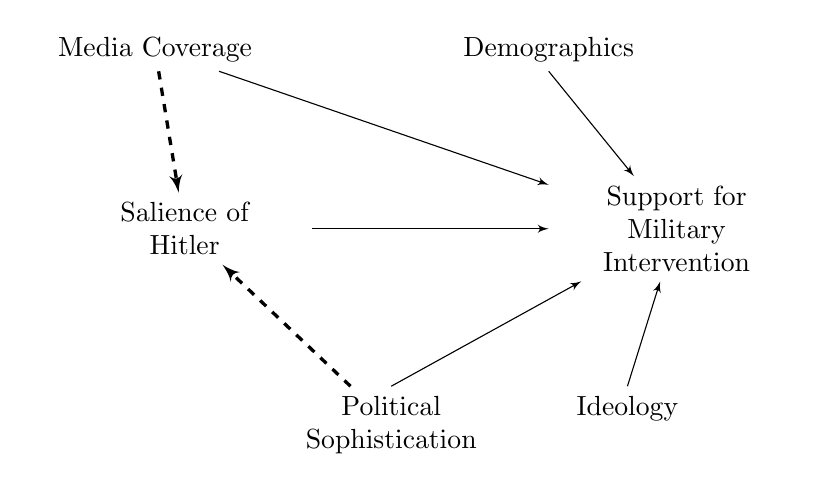
\begin{tikzpicture}[>=latex',circ/.style={draw, shape=circle, node distance=5cm, line width=1.5pt}]
    \draw (0,0) node[left, text width=3cm, align=center] (X) {Salience of\\Hitler};
    \draw[->] (X) -- (3,0) node[right, text width=3cm, align=center] (Y) {Support for\\Military\\Intervention};
    \draw (-2,2) node[above, text width=3cm, align=center] (Z) {Media Coverage};
    \draw[->] (Z) -- (Y);
    \draw[->] (3,2) node[above] (A) {Demographics} -- (Y);
    \draw[->] (4,-2) node[below] (B) {Ideology} -- (Y);
    \draw[->] (1,-2) node[below, text width=3cm, align=center] (E) {Political\\Sophistication} -- (Y);
	\draw<2->[->, dashed, very thick] (Z) -- (X);
	\draw<3->[->, dashed, very thick] (E) -- (X);
\end{tikzpicture}
\end{center}
\end{frame}


\frame{

\frametitle{Experiments are different}

\begin{enumerate}\itemsep0.75em
\item<2-> Causal inferences from \textit{design} not \textit{analysis}
\item<3-> Solves both temporal ordering and confounding
	\begin{itemize}
   		\item Treatment ($X$)  applied by researcher before outcome ($Y$)
   		\item Randomization eliminates confounding ($\mathbf{Z}$)
   		\item We don't need to ``control'' for anything
	\end{itemize}
\item<4-> Basically: $Y = \beta_0 + \beta_1 X + \epsilon $
\item<5-> Thus experiments are a ``gold standard''
\end{enumerate}

}


% Mill's method of difference
\frame{
\frametitle{{\normalsize Mill's Method of Difference}}

\small

If an instance in which the phenomenon under investigation occurs, and an instance in which it does not occur, \textbf<2->{have every circumstance save one in common}, that one occurring only in the former; \textbf<2->{the circumstance in which alone the two instances differ, is the} effect, or \textbf<2->{cause}, or an necessary part of the cause, \textbf<2->{of the phenomenon}.
}


\questions


\frame{

\frametitle{Neyman-Rubin Potential Outcomes Framework}

If we are interested in some outcome $Y$, then for every unit $i$, there are numerous ``potential outcomes'' $Y*$ only one of which is visible in a given reality. Comparisons of (partially unobservable) potential outcomes indicate causality.

}

\frame{

\frametitle{Neyman-Rubin Potential Outcomes Framework}

Concisely, we typically discuss two potential outcomes:

\begin{itemize}\small
\item $Y_{0i}$, the \textit{potential} outcome \textit{realized} if $X_i = 0$ (b/c $D_i = 0$, assigned to control)
\item $Y_{1i}$, the \textit{potential} outcome \textit{realized} if $X_i = 1$ (b/c $D_i = 1$, assigned to treatment)
\end{itemize}

}



% design-based experimental inference
\frame{
	\frametitle{Experimental Inference I}
	\small
	\begin{itemize}\itemsep0.5em
    	\item<1-> Each unit has multiple \textit{potential} outcomes, but we only observe one of them, randomly
    	\item<2-> In this sense, we are sampling potential outcomes from each unit's population of potential outcomes
		\only<2->{
			\begin{center}
			\begin{tabular}{ccccc}
			unit & low & high & \onslide<3->{control} & \onslide<4->{etc.} \\ \midrule
			1 & ? & ? & \onslide<3->{?} & \onslide<4->{\dots} \\
			2 & ? & ? & \onslide<3->{?} & \onslide<4->{\dots} \\
			3 & ? & ? & \onslide<3->{?} & \onslide<4->{\dots} \\
			4 & ? & ? & \onslide<3->{?} & \onslide<4->{\dots} \\ \bottomrule
			\end{tabular}
			\end{center}
		}
	\end{itemize}
}

\frame{
	\frametitle{Experimental Inference II}
	\small
	\begin{itemize}\itemsep0.5em
    	\item<1-> We cannot see individual-level causal effects
    	\item<2-> We can see \textit{average causal effects}
    		\begin{itemize}
        		\item<2-> Ex.: Average difference in military support among those thinking of Hitler versus not
    		\end{itemize}
    	\item<3-> We want to know: $TE_i = Y_{1i} - Y_{0i}$
	\end{itemize}
}

\frame{
	\frametitle{Experimental Inference III}
	\small
	\begin{itemize}\itemsep0.5em
		\item<1-> We want to know: $TE_i = Y_{1i} - Y_{0i}$ for every $i$ in the population
		\item<2-> We can average: $E[TE_i] = E[Y_{1i} - Y_{0i}] = E[Y_{1i}] - E[Y_{0i}]$
		\item<3-> But we still only see one potential outcome for each unit:\\ \vspace{1em}
    		$ATE_{naive} = E[Y_{1i} | X = 1] - E[Y_{0i} | X = 0]$
    	\item<4-> Is this what we want to know?
	\end{itemize}
}


\frame{
	\frametitle{Experimental Inference IV}
	\small
	\begin{itemize}\itemsep0.5em
	\item What we want and what we have:
		\begin{align}
		ATE & = E[Y_{1i}] - E[Y_{0i}] \\[1em]
		ATE_{naive} & = E[Y_{1i} | X = 1] - E[Y_{0i} | X = 0]
		\end{align}		
	\item<2-> Are the following statements true?\\
  		\begin{itemize}\itemsep0.5em
      		\item<2-> $E[Y_{1i}] = E[Y_{1i} | X = 1]$
      		\item<2-> $E[Y_{0i}] = E[Y_{0i} | X = 0]$
  		\end{itemize}
  	\item<3-> Not in general!
  	\end{itemize}
}

\frame{
	\frametitle{Experimental Inference V}
	\small
	\begin{itemize}\itemsep0.5em
    	\item Only true when both of the following hold:
    	\begin{align}
    	E[Y_{1i}] = E[Y_{1i} | X = 1] = E[Y_{1i} | X = 0]\\
    	E[Y_{0i}] = E[Y_{0i} | X = 1] = E[Y_{0i} | X = 0]
    	\end{align}
    	\item In that case, potential outcomes are \textit{independent} of treatment assignment
		\item If true (e.g., due to randomization of $X$), then:
    	\begin{align*}
    	ATE_{naive} & = E[Y_{1i} | X = 1] - E[Y_{0i} | X = 0] \tag{5}\\
    	& = E[Y_{1i}] - E[Y_{0i}]\\
    	& = ATE
    	\end{align*}
	\end{itemize}
}

\frame{
	\frametitle{Experimental Inference VI}
	
	\begin{itemize}\itemsep1em
    	\item This holds in experiments because of a \textit{physical process of randomization}\footnote{Random means ``known probability of treatment'' not ``haphazard''.}
   		\item<2-> Units differ only in side of coin that was up
	   		\begin{itemize}\footnotesize
	   		\item $X_i = 1$ only because $D_i = 1$
	   		\end{itemize}
	   	\item<3-> Implications:
		   	\begin{itemize}
		   	\item Covariate balance
		   	\item Potential outcomes balanced and independent of treatment assignment
		   	\item No confounding (selection bias)
		   	\end{itemize}
	\end{itemize}
}




\begin{frame}
\begin{center}
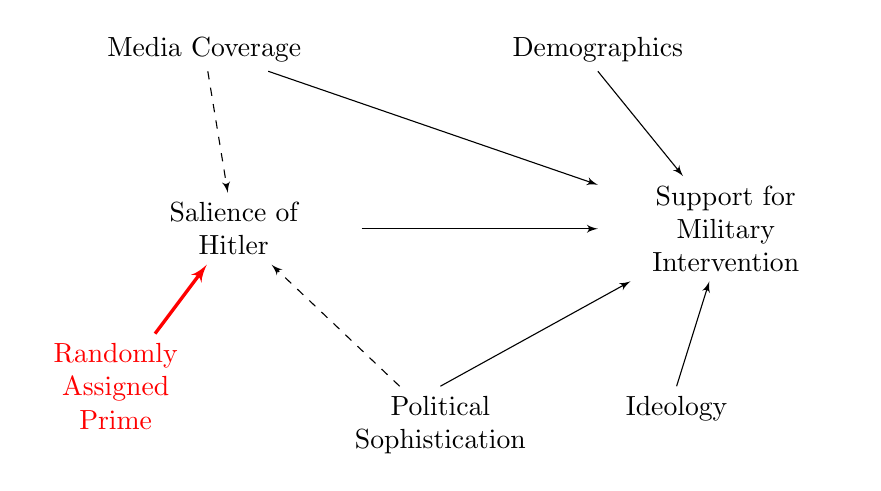
\begin{tikzpicture}[>=latex',circ/.style={draw, shape=circle, node distance=5cm, line width=1.5pt}]
    \draw (0,0) node[left, text width=3cm, align=center] (X) {Salience of\\Hitler};
    \draw[->] (X) -- (3,0) node[right, text width=3cm, align=center] (Y) {Support for\\Military\\Intervention};
    \draw (-2,2) node[above, text width=3cm, align=center] (Z) {Media Coverage};
    \draw[->] (Z) -- (Y);
    \draw[->] (3,2) node[above] (A) {Demographics} -- (Y);
    \draw[->] (4,-2) node[below] (B) {Ideology} -- (Y);
    \draw[->] (1,-2) node[below, text width=3cm, align=center] (E) {Political\\Sophistication} -- (Y);
	\draw[->, dashed] (E) -- (X);
	\draw[->, dashed] (Z) -- (X);
	\draw<2-> (-2,-2) node[left, color=red, text width=2cm, align=center] (T) {Randomly\\Assigned\\Prime};
	\draw<2->[->, very thick, color=red] (T) -- (X);
\end{tikzpicture}
\end{center}
\end{frame}


\questions



\frame{
\frametitle{Experimental Analysis I}
\small
\begin{itemize}
\item The statistic of interest in an experiment is the \textit{sample average treatment effect} (SATE)
\item If our sample is \textit{representative}, then this provides an estimate of the population average treatment (PATE)
	\begin{itemize}
	\item Design-based random sampling
	\item Model-based re-weighting
	\end{itemize}
\item<2-> This boils down to being a mean-difference between two groups:
	\begin{equation}
	SATE = \frac{1}{n_1}\sum Y_{1i} - \frac{1}{n_0}\sum Y_{0i}
	\end{equation}
\end{itemize}
}



\frame[label=tidy]{

\frametitle{Tidy Experimental Data}

An experimental data structure looks like:

\small

\begin{center}
\begin{tabular}{ccc}
\texttt{unit} & \texttt{treatment} & \texttt{outcome} \\ \hline 
1 & 0 & 13 \\
2 & 0 & 6 \\
3 & 0 & 4 \\
4 & 0 & 5 \\
5 & 1 & 3 \\
6 & 1 & 1 \\
7 & 1 & 10 \\
8 & 1 & 9 \\ \hline
\end{tabular}
\end{center}

}

\frame{

\frametitle{Tidy Experimental Data}

Sometimes it looks like this instead, which is bad:

\small

\begin{center}
\begin{tabular}{cccc}
\texttt{unit} & \texttt{treatment} & \texttt{outcome0}  & \texttt{outcome1} \\ \hline 
1 & 0 & 13 & NA \\
2 & 0 & 6 & NA \\
3 & 0 & 4 & NA \\
4 & 0 & 5 & NA \\
5 & 1 & NA & 3 \\
6 & 1 & NA & 1 \\
7 & 1 & NA & 10 \\
8 & 1 & NA & 9 \\ \hline
\end{tabular}
\end{center}

}

\againframe{tidy}


\frame{

\frametitle{Computation of Effects I}

\begin{itemize}\itemsep0.5em
\item In practice we often estimate SATE using t-tests, ANOVA, or OLS regression
\item These are all basically equivalent
\item<2-> Reasons to choose one procedure over another:
	\begin{itemize}
	\item<2-> Disciplinary norms
	\item<3-> Ease of interpretation
	\item<4-> Flexibility for >2 treatment conditions
	\end{itemize}
\end{itemize}

}



\begin{frame}[fragile]

\frametitle{Computation of Effects II}

R:\small
\begin{verbatim}
t.test(outcome ~ treatment, data = data)
lm(outcome ~ factor(treatment), data = data)
\end{verbatim}

\vspace{1em}

Stata:\small
\begin{verbatim}
ttest outcome, by(treatment)
reg outcome i.treatment
\end{verbatim}

\end{frame}


\questions

\frame{
\frametitle{Experimental Analysis II}
	\small
\begin{itemize}\itemsep0.5em
\item We don't just care about the size of the SATE. We also want to know whether it is significantly different from zero (i.e., different from no effect/difference)
\item Thus we need to estimate the \textit{variance} of the SATE
\item The variance is influenced by:
	\begin{itemize}
	\item Total sample size
	\item Element variance of the outcome, $Y$
	\item Relative size of each treatment group
	\item (Some other factors)
	\end{itemize}
\end{itemize}
}


\frame{
\frametitle{Experimental Analysis III}
	\small
\begin{itemize}\itemsep0.5em
\item Formula for the variance of the SATE is:\\

$\widehat{Var}(SATE) = \dfrac{\widehat{Var}(Y_0)}{n_0} + \dfrac{\widehat{Var}(Y_1)}{n_1}$

	\begin{itemize}
	\item $\widehat{Var}(Y_0)$ is control group variance
	\item $\widehat{Var}(Y_1)$ is treatment group variance
	\end{itemize}

\item We often express this as the \textit{standard error} of the estimate:\\
$\widehat{SE}_{SATE} = \sqrt{\frac{\widehat{Var}(Y_0)}{n_0} + \frac{\widehat{Var}(Y_1)}{n_1}}$
\end{itemize}
}


\frame{

\frametitle{Intuition about Variance}

\begin{itemize}\itemsep1em
\item Bigger sample $\rightarrow$ smaller SEs
\item Smaller variance $\rightarrow$ smaller SEs
\item Efficient use of sample size:
	\begin{itemize}
	\item When treatment group variances equal, equal sample sizes are most efficient
	\item When variances differ, sample units are better allocated to the group with higher variance in \emph{Y}
	\end{itemize}
\end{itemize}


}



\frame{

\frametitle{Statistical Power}

\begin{itemize}\itemsep0.5em
\item Power analysis is used to determine sample size before conducting an experiment

\item Type I and Type II Errors

\begin{center}
\begin{tabular}{lcc}
\toprule
& $H_0$ False & $H_0$ True \\ 
& ($|ATE| > 0$) & ($ATE = 0$) \\ \midrule
Reject $H_0$ & \textbf{True positive} & Type I Error \\
Accept $H_0$ & Type II Error & True zero \\ \bottomrule
\end{tabular}
\end{center}

	\begin{itemize}
	\item True positive rate ($1-\kappa$) is power
	\item False positive rate is the significance threshold ($\alpha$)
	\end{itemize}

\end{itemize}
}


\frame{

\frametitle{Doing a Power Analysis}

\begin{itemize}
\item $\mu$, Treatment group mean outcomes
\item $N$, Sample size
\item $\sigma$, Outcome variance
\item $\alpha$ Statistical significance threshold
\item $\phi$, a sampling distribution
\end{itemize}

$Power = \phi\left( \frac{|\mu_1 - \mu_0|\sqrt{N}}{2\sigma} - \phi^{-1}\left( 1 - \frac{\alpha}{2} \right) \right)$

}



\frame{
\frametitle{Intuition about Power}

Minimum detectable effect is the smallest effect we could detect given sample size, ``true'' ATE, variance of outcome measure, power ($1-\kappa$), and $\alpha$.\\

\vspace{1em}

\only<2->{In essence: some non-zero effect sizes are not detectable by a study of a given sample size.}

\vspace{1em}

\only<3->{In underpowered study, we will be unlikely to detect true small effects. And most effects are small! \footnote{Gelman, A. and Weakliem, D. 2009. ``Of Beauty, Sex and Power.'' \textit{American Scientist} 97(4): 310--16}}

}


\frame{

\frametitle{Intuition about Power}

\begin{itemize}\itemsep1em
\item It can help to think in terms of ``standardized effect sizes''
\item Intuition: How large is the effect in standard deviations of the outcome?
	\begin{itemize}
	\item Know if effects are large or small
	\item Compare effects across studies
	\end{itemize}
\item<2-> Cohen's $d$:\\ $d = \frac{\bar{x}_1 - \bar{x}_0}{s}$, where
$s = \sqrt{\frac{(n_1 - 1)s_1^2 + (n_0 - 1)s_0^2}{n_1 + n_0 - 2}}$
\item<3-> Small: 0.2; Medium: 0.5; Large: 0.8
\end{itemize}

}

\frame{
\frametitle{Intuition about Power}

\begin{center}
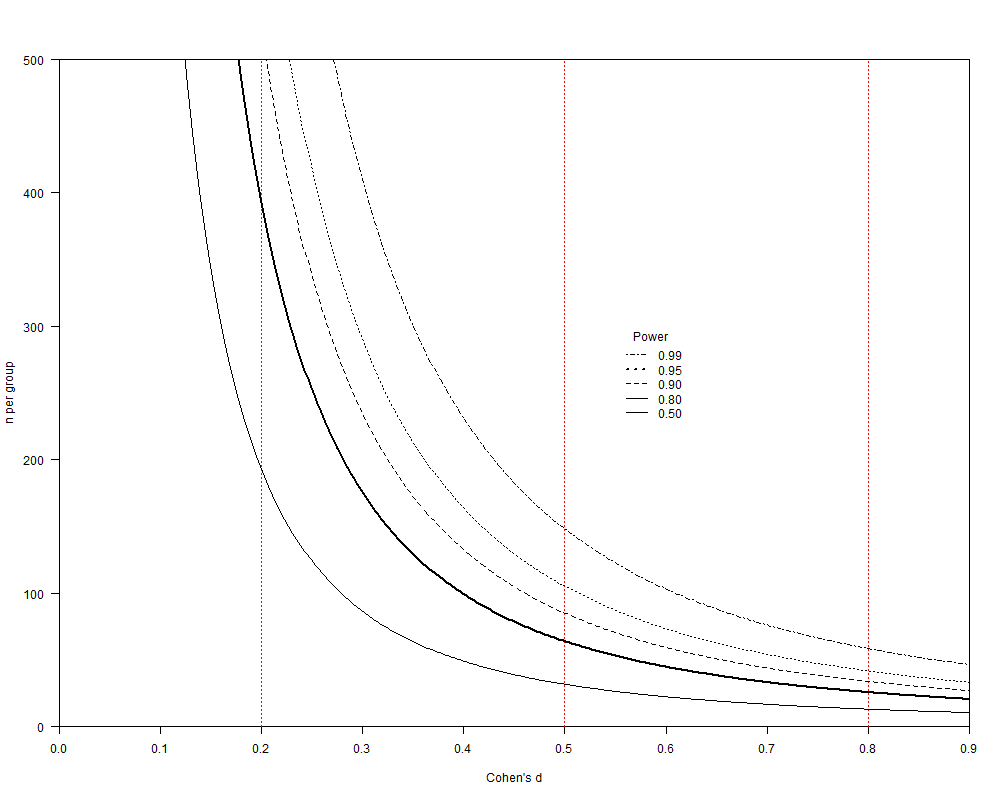
\includegraphics[height=0.8\textheight, trim = 0in 0in 0in 0.5in , clip]{images/power}
\end{center}

}


\begin{frame}[fragile]

\frametitle{Power analysis in R}
\small
\begin{verbatim}
power.t.test(
  # sample size (leave blank!)
  n = ,
  
  # minimum detectable effect size
  delta = 0.4, sd = 1,
  
  # alpha and power (1-kappa)
  sig.level = 0.05, power = 0.8,
  
  # two-tailed vs. one-tailed test
  alternative = "two.sided"
)
\end{verbatim}
\end{frame}


\begin{frame}[fragile]

\frametitle{Power analysis in Stata}
\small
\begin{verbatim}
power twomeans 0, diff(0.2)

// for multiple values of 
forvalues i = 0.1 (0.1) 1.0 {
    power twomeans 0, diff(`i')
}

// using raw effect sizes and standard deviations
power twomeans 0 0.5, sd1(.5) sd2(.7)

// adjusting alpha or power
power twomeans 0, diff(0.2) alpha(0.10) power(0.7)
\end{verbatim}
\end{frame}



\begin{frame}

\frametitle{Increasing/Decreasing Power}

\begin{columns}
\begin{column}{0.5\textwidth}
\begin{block}{Increases Power}
\begin{itemize}\itemsep1em
\item Bigger sample
\item Precise measures
\item Covariates?
\end{itemize}
\end{block}
\end{column}

\begin{column}{0.5\textwidth}
\begin{block}{Decreases Power}
\begin{itemize}\itemsep1em
\item Attrition
\item Noncompliance
\item Clustering
\end{itemize}
\end{block}
\end{column}
\end{columns}

\end{frame}




\frame{}


\frame{

\frametitle{Factorial Designs}

\begin{itemize}\itemsep1em
\item The two-condition experiment is a stylized ideal

\item An experiment can have any number of conditions
	\begin{itemize}\footnotesize
	\item Up to the limits of sample size
	\item More than 8--10 conditions is typically unwieldy
	\end{itemize}

\item Three ``flavors'':
	\begin{itemize}
	\item Multiple conditions in a single factor
	\item Multiple fully \textit{crossed} factors
	\item Partially crossed (``fractional factorial'') designs
	\end{itemize}

\item Regression methods provide a generalizable tool for causal inference in such designs
\end{itemize}
}

\begin{frame}
\begin{center}
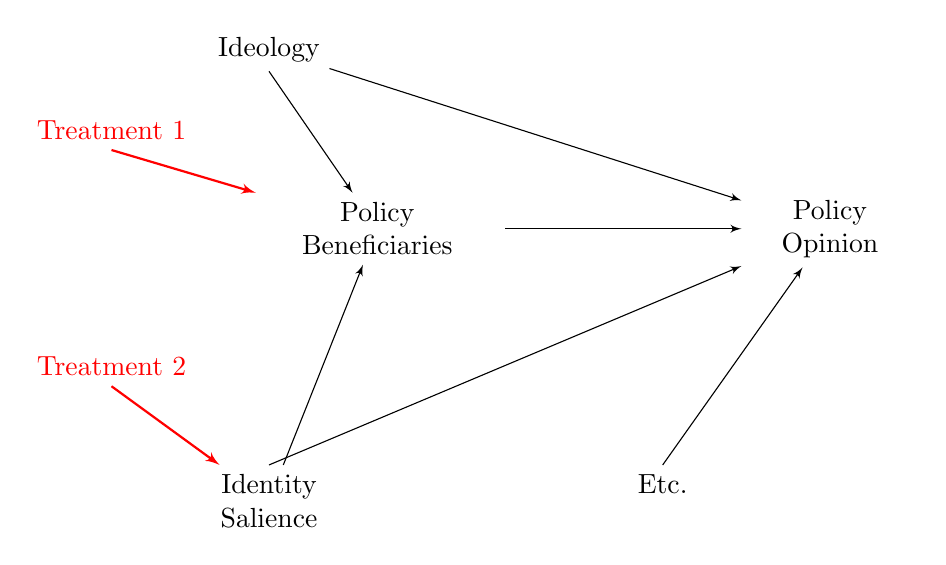
\begin{tikzpicture}[>=latex',circ/.style={draw, shape=circle, node distance=5cm, line width=1.5pt}]
    \draw (0,0) node[left, text width=3cm, align=center] (X) {Policy\\Beneficiaries};
    \draw[->] (X) -- (3,0) node[right, text width=2cm, align=center] (Y) {Policy\\Opinion};
    \draw[->] (-3,2) node[above] (Z) {Ideology} -- (X);
    \draw[->] (Z) -- (Y);
    \draw[->] (2,-3) node[below, text width=3cm, align=center] (E) {Etc.} -- (Y);
    \draw[->] (-3, -3) node[below, text width=2.5cm, align=center] (W) {Identity Salience} -- (Y);
    \draw[->] (W) -- (X);
    \draw<2->[->,thick,red] (-5,1) node[above] (T1) {Treatment 1} -- (X);
    \draw<2->[->,thick,red] (-5,-2) node[above] (T1) {Treatment 2} -- (W);
\end{tikzpicture}
\end{center}
\end{frame}


\frame{
	\frametitle{{\normalsize Example\footnote{Transue. 2007. ``Identity Salience, Identity Acceptance, and Racial Policy Attitudes: {American} National Identity as a Uniting Force.'' \textit{American Journal of Political Science} 51(1): 78--91.}}}
	

\begin{itemize}\itemsep1em
\item \only<1,3>{How close do you feel to your ethnic or racial group?}\only<2,4>{How close do you feel to other Americans?}
\item \only<1-2>{Some people have said that taxes need to be raised to take care of pressing national needs. How willing would you be to have your taxes raised to improve education in public schools?}\only<3-4>{Some people have said that taxes need to be raised to take care of pressing national needs. How willing would you be to have your taxes raised to improve educational opportunities for minorities?}
\end{itemize}
	
}


\frame{

\frametitle{2x2 Factorial Design}

\only<1>{
\begin{center}
\begin{tabular}{lr}
Condition &  \\ \midrule
Educ. for Minorities & $Y_1$ \\
Schools & $Y_0$ \\ \bottomrule
\end{tabular}
\end{center}
}

\only<2>{
\begin{center}
\begin{tabular}{lrr}
Condition & Americans & Own Race \\ \midrule
Educ. for Minorities & $Y_{1,0}$ & $Y_{1,1}$ \\
Schools & $Y_{0,0}$ & $Y_{0,1}$ \\ \bottomrule
\end{tabular}
\end{center}
}

}


\frame{

\frametitle{Two ways to \textit{parameterize} this}

Dummy variable regression (i.e., treatment--control CATEs):

$Y = \beta_0 + \beta_1 X_{0,1} + \beta_2 X_{1,0} + \beta_3 X_{1,1} + \epsilon$

\vspace{1em}

Interaction effects (i.e., treatment--treatment CATEs):

$Y = \beta_0 + \beta_1 X1_{1} + \beta_2 X2_{1} + \beta_3 X1_1 * X2_1 + \epsilon$

\vspace{1em}

Use \texttt{margins} to extract marginal effects

}


\frame<1>[label=factorialconsiderations]{

\frametitle{Considerations}

\begin{itemize}\itemsep0.5em
\item Factorial designs can quickly become unwieldy and expensive
\item<2-> Need to consider what CATEs are of theoretical interest
	\begin{itemize}
	\item Treatment--control, pairwise
	\item Treatment--treatment, pairwise
	\item Marginal effects, averaging across other factors
	\item Comparison of merged conditions
	\end{itemize}
\end{itemize}

}

\frame{

\frametitle{Probably obvious, but\dots}

\footnotesize

\begin{center}
\begin{tabular}{cccc}
Factors & Conditions per factor & Total Conditions & $n$ \\ \midrule
1 & 2 & 2 & 400 \\ 
1 & 3 & 3 & 600 \\
1 & 4 & 4 & 800 \\
2 & 2 & 4 & 800 \\
2 & 3 & 6 & 1200 \\
2 & 4 & 8 & 1600 \\
3 & 3 & 9 & 1800 \\
3 & 4 & 12 & 2400 \\
4 & 4 & 16 & 3200 \\ \bottomrule
\end{tabular}
\end{center}

{\footnotesize Assumes power to detect a relatively small effect, but no consideration of multiple comparisons.}

}

\againframe{factorialconsiderations}

% marginal effects of factors are marginal across the set of levels of the other factors; if those factors aren't complete, then external validity problem


\questions




\frame{}


\section[Theory]{From Theory to Design}
\frame{\tableofcontents[currentsection,subsubsectionstyle=hide]}
% deriving hypotheses from theory and manipulations from hypotheses

\subsection{Translating Hypotheses into Designs}
\frame{\tableofcontents[currentsection,currentsubsection,subsubsectionstyle=hide]}


\frame{

\frametitle{From Theory to Design}

\begin{itemize}\itemsep1em
\item From theory, we derive testable hypotheses
\begin{itemize}
\item Hypotheses are expectations about differences in outcomes across levels of a putatively causal variable
\end{itemize}
\item Hypothesis must be testable by an SATE ($H_0=0$)
\item Manipulations are developed to create variation in that causal variable
\end{itemize}

}


\frame{

\frametitle{{\normalsize Example: News Framing}}

\small

\begin{itemize}
\item Theory: Presentation of news affects opinion
\item Hypotheses:
	\begin{itemize}\footnotesize
	\item News emphasizing free speech increases support for a hate group rally
	\item News emphasizing public safety decreases support for a hate group rally
	\end{itemize}
\item Manipulation:
	\begin{itemize}\footnotesize
	\item Control group: no information
	\item Free speech group: article emphasizing rights
	\item Public safety group: article emphasizing safety
	\end{itemize}
\end{itemize}

}




\frame{

\frametitle{{\normalsize Example: Partisan Identity}}

\small

\begin{itemize}
\item Theory: Strength of partisan identity affects tendency to accept party position
\item Hypotheses:
	\begin{itemize}\small
	\item Strong partisans are more likely to accept their party's position on an issue
	\end{itemize}
\item Manipulation:
	\begin{itemize}\small
	\item Control group: no manipulation
	\item ``Univalent'' condition
	\item ``Ambivalent'' condition
	\end{itemize}
\end{itemize}

}


\frame[label=ambivalentpartisan]{

\frametitle{\textbf{\only<1>{Univalent}\only<2>{Ambivalent}}}

These days, Democrats and Republicans differ from one another considerably. The two groups seem to be growing further and further apart, not only in terms of their opinions but also their lifestyles. Earlier in the survey, you said you tend to identify as a \textit{Democrat/ Republican}. Please take a few minutes to think about what you like about \textit{Democrats/ Republicans} compared to the \textit{Republicans/ Democrats}. Think of 2 to 3 things you especially like best about \textbf{\only<1>{your party}\only<2>{the other party}}. Then think of 2 to 3 things you especially dislike about \textbf{\only<2>{your party}\only<1>{the other party}}. Now please write those thoughts in the space below.

}



\frame{

\frametitle{Treatments Test Hypotheses!}

\begin{itemize}\itemsep1em
\item<2-> Experimental ``factors'' are expressions of hypotheses as randomized groups
\item<3-> What stimulus each group receives depends on hypotheses
\item<4-> Three ways hypotheses lead to stimuli:
	\begin{itemize}
	\item presence/absence
	\item levels/doses
	\item qualitative variations
	\end{itemize}
\end{itemize}

}


\frame{

\frametitle{{\normalsize Ex.: Presence/Absence}}

\small

\begin{itemize}\itemsep0.5em
\item Theory: Negative campaigning reduces support for the party described negatively.
\item Hypothesis: Exposure to a negative advertisement criticizing a party reduces support for that party.
\item Manipulation:
	\begin{itemize}\small 
	\item Control group receives no advertisement. 
	\item Treatment group watches a video containing a negative ad describing a party.
	\end{itemize}
\end{itemize}

}


\frame{

\frametitle{{\normalsize Ex.: Levels/doses}}

\small

\begin{itemize}\itemsep-0.2em
\item Theory: Negative campaigning reduces support for the party described negatively.
\item Hypothesis: Exposure to higher levels of negative advertising criticizing a party reduces support for that party.
\item Manipulation:
	\begin{itemize}\footnotesize
	\item Control group receives no advertisement. 
	\item Treatment group 1 watches a video containing 1 negative ad describing a party.
	\item Treatment group 2 watches a video containing 2 negative ads describing a party.
	\item Treatment group 3 watches a video containing 3 negative ads describing a party.
	\item etc.
	\end{itemize}
\end{itemize}

}


\frame{

\frametitle{{\normalsize Ex.: Qualitative variation}}

\small

\begin{itemize}
\item Theory: Negative campaigning reduces support for the party described negatively.
\item Hypothesis: Exposure to a negative advertisement criticizing a party reduces support for that party, while a positive advertisement has no effect.
\item Manipulation:
	\begin{itemize}\footnotesize
	\item Control group receives no advertisement. 
	\item Negative treatment group watches a video containing a negative ad describing a party.
	\item Positive treatment group watches a video containing a positive ad describing a party.
	\end{itemize}
\end{itemize}

}

\questions


\subsection{Assessing Quality}
\frame{\tableofcontents[currentsection,currentsubsection,subsubsectionstyle=hide]}

\frame{

\frametitle{Activity!}

\begin{itemize}\itemsep0.5em
\item How do we know if an experiment is any good?
\item Talk with a partner for about 3 minutes
\item Try to develop some criteria that allow you to evaluate ``what makes for a good experiment?'' 
\end{itemize}

}


\frame{

\frametitle{Some possible criteria}

\small

\begin{itemize}\itemsep-0.2em
\item Significant results
\item Face validity
\item Coherent for respondents
\item Non-obvious to respondents
\item Simple
\item Indirect/unobtrusive
\item Validated by prior work
\item Innovative/creative
\item \dots
\end{itemize}

}


\frame{

\begin{quote}\large
The best criterion for evaluating the quality of an experiment is whether it manipulated the intended independent variable and controlled everything else by design.
\end{quote}
\onslide<2->{\small\hspace{5em} --Thomas J. Leeper (5 February 2018)}

}

\frame{

\frametitle{How do we know we manipulated what we think we manipulated?}

\small

\begin{itemize}
\item<2-> Outcomes are affected consistent with theory
\item<3-> Before the study using \textit{pilot testing} (or \emph{pretesting})
\item<4-> During the study, using \emph{manipulation checks}
\item<5-> During the study, using \emph{placebos}
\item<6-> During the study, using \textit{non-equivalent outcomes}
\end{itemize}
}

\frame{

\frametitle{I. Outcomes Affected}

\begin{itemize}\itemsep0.5em
\item Follows a circular logic!
\item Doesn't tell us anything if we hypothesize null effects
\end{itemize}

}


\frame{

\frametitle{II. Pilot Testing}

\small

\begin{itemize}\itemsep0.2em
\item Goal: establish construct validity of manipulation
\item Assess whether a set of possible manipulations affect a measure of the \textit{independent} variable
\item<2-> Example:
	\begin{itemize}
	\item Goal: Manipulate the ``strength'' of an argument
	\item Write several arguments
	\item Ask pilot test respondents to report how strong each one was
	\end{itemize}
\end{itemize}

}

\frame{

\frametitle{III. Manipulation Checks}

\small

\begin{itemize}\itemsep0.2em
\item Manipulation checks are items added post-treatment, post-outcome that assess whether the \textit{independent} variable was affected by treatment
\item We typically talk about manipulations as directly setting the value of $X$, but in practice we are typically manipulating something \textit{that we think} strongly modifies $X$
\item<2-> Example: information manipulations aim to modify knowledge or beliefs, but are necessarily imperfect at doing so
\end{itemize}

}

\frame{

\frametitle{\normalsize Manipulation check example\footnote{Leeper \& Slothuus. n.d. ``Can Citizens Be Framed?'' Available from: \url{http://thomasleeper.com/research.html}.}}

\begin{enumerate}
\item Treatment 1: Supply Information
\item Manipulation check 1: measure beliefs
\item Treatment 2: Prime a set of considerations
\item Outcome: Measure opinion
\item Manipulation check 2: measure dimension salience
\end{enumerate}

}


\frame{

\frametitle{{\normalsize Some Best Practices}}


\begin{itemize}\itemsep0.5em
\item<2-> Manipulation checks should be innocuous
	\begin{itemize}
	\item Shouldn't modify independent variable
	\item Shouldn't modify outcome variable
	\end{itemize}
\item<3-> Generally, measure post-outcome
\item<4-> Measure both what you wanted to manipulate \textit{and} what you didn't want to manipulate
	\begin{itemize}
	\item Most treatments are \textit{compound}!
	\end{itemize}
\end{itemize}

}

\frame{

\frametitle{IV. Placebos}

\begin{itemize}\itemsep0.5em
\item Include an experimental condition that \textit{does not} manipulate the variable of interest (but might affect the outcome)
\item<2-> Example:
	\begin{itemize}
	\item Study whether risk-related arguments about climate change increase support for a climate change policy
	\item Placebo condition: control article with risk-related arguments about non-environmental issue (e.g., terrorism)
	\end{itemize}
\end{itemize}

}

\frame{

\frametitle{V. Non-equivalent outcomes}

\small

\begin{itemize}\itemsep0.5em
\item Measures an outcome that \textit{should not} be affected by independent variable
\item<2-> Example:
	\begin{itemize}
	\item Assess effect of some treatment on attitudes toward group A
	\item Focal outcome: attitudes toward group A
	\item Non-equivalent outcome: attitudes toward group B
	\end{itemize}
\end{itemize}

}


\frame{

\frametitle{{\normalsize Aside: Demand Characteristics}}

\small

\begin{itemize}\itemsep0.5em
\item ``Demand characteristics'' are features of experiments that (unintentionally) imply the purpose of the study and thereby change respondents' behavior (to be consistent with theory)
\item<2-> Implications:
	\begin{itemize}\footnotesize
	\item Design experimental treatments that are non-obvious
	\item Do not disclose the purpose of the study up front\footnote{But, consider the ethics of not doing so (more Friday)}
	\end{itemize}
\end{itemize}

}




\subsection[Examples]{Common Paradigms and Examples}
\frame{\tableofcontents[currentsection,currentsubsection,subsubsectionstyle=hide]}


\frame{

\frametitle{Question Wording Designs}

\begin{itemize}\itemsep1em
\item Simplest paradigm for presence/absence or qualitative variation
\item Manipulation operationalizes this by asking two different questions
\item Outcome is the answer to the question
\item Example: Schuldt et al. ```Global Warming' or `Climate Change'? Whether the Planet is Warming Depends on Question Wording.''
\end{itemize}

}

\frame{

\small

You may have heard about the idea that the world's temperature may have been \textbf{\only<1>{going up}\only<2>{changing}} over the past 100 years, a phenomenon sometimes called \textbf{\only<1>{global warming}\only<2>{climate change}}. What is your personal opinion regarding whether or not this has been happening?
	\begin{itemize}\itemsep-0.25em\footnotesize
	\item Definitely has not been happening
	\item Probably has not been happening
	\item Unsure, but leaning toward it has not been happening
	\item Not sure either way
	\item Unsure, but leaning toward it has been happening
	\item Probably has been happening
	\item Definitely has been happening
	\end{itemize}
}


\frame{

\frametitle{{\normalsize Another framing example\footnote{Singer \& Couper. 2014. ``The Effect of Question Wording on Attitudes toward Prenatal Testing and Abortion.'' \textit{Public Opinion Quarterly} 78(3): 751--760.}}}

\footnotesize

Today, tests are being developed that make it possible to detect serious genetic defects \textbf{\only<1>{before a baby is born}\only<2>{in the fetus during pregnancy}}. But so far, it is impossible either to treat or to correct most of them. If (you/your partner) were pregnant, would you want (her) to have a test to find out if the \textbf{\only<1>{baby}\only<2>{fetus}} has any serious genetic defects? (Yes/No)\\

\vspace{0.5em}

Suppose a test shows the \textbf{\only<1>{baby}\only<2>{fetus}} has a serious genetic defect. Would you, yourself, want (your partner) to have an abortion if a test shows the \textbf{\only<1>{baby}\only<2>{fetus}} has a serious genetic defect? (Yes/No)

}


\frame{

\frametitle{{\normalsize Another framing example\footnote{Bobo \& Johnson. 2004. ``A Taste for Punishment: Black and White Americans' Views on the Death Penalty and the War on Drugs.'' Du Bois Review 1(1): 151--180.}}}

\only<2>{Blacks are about 12\% of the U.S. population, but they were half of the homicide offenders last year. }Do you favor or oppose the death penalty for persons convicted of murder?

}

\frame{

\frametitle{{\normalsize Another framing example\footnote{Haider-Markel \& Joslyn. 2001. ``Gun Policy, Opinion, Tragedy, and Blame Attribution: The Conditional Influence of Issue Frames.'' \textit{Journal of Politics} 63(2): 520--543.}}}

\only<1>{Concealed handgun laws have recently received national attention. Some people have argued that law-abiding citizens have the right to protect themselves.}\only<2>{Concealed handgun laws have recently received national attention. Some people have argued that laws allowing citizens to carry concealed handguns threaten public safety because they would allow almost anyone to carry a gun almost anywhere, even onto school grounds.} What do you think about concealed handgun laws?

}





\frame{

\frametitle{{\normalsize Question Order Designs}}

\small

\begin{itemize}
\item Manipulation of pre-outcome questionnaire
\item<2-> Example:
	\begin{itemize}
	\item Goal: assess influence of value salience on support for a policy
	\item Manipulate by asking different questions:
		\begin{itemize}
		\item Battery of 5 ``rights'' questions, or
		\item Battery of 5 ``life'' questions
		\end{itemize}
	\item Measure support for legalized abortion
	\end{itemize}
\item<3-> If answers to manipulated questions matter, can measure rest post-outcome
\end{itemize}

}

\frame{
	\frametitle{{\normalsize Ex. Question-as-treatment\footnote{Transue. 2007. ``Identity Salience, Identity Acceptance, and Racial Policy Attitudes: {American} National Identity as a Uniting Force.'' \textit{American Journal of Political Science} 51(1): 78--91.}}}
	

\begin{itemize}
\item \only<1,3>{How close do you feel to your ethnic or racial group?}\only<2,4>{How close do you feel to other Americans?}
\item \only<1-2>{Some people have said that taxes need to be raised to take care of pressing national needs. How willing would you be to have your taxes raised to improve education in public schools?}\only<3-4>{Some people have said that taxes need to be raised to take care of pressing national needs. How willing would you be to have your taxes raised to improve educational opportunities for minorities?}
\end{itemize}
	
}


\frame{

\frametitle{{\normalsize Ex.: Knowledge and Political Interest}}

\footnotesize

\begin{enumerate}
\item Do you happen to remember anything special that your U.S. Representative has done for your district or for the people in your district while he has been in Congress?
\item Is there any legislative bill that has come up in the House of Representatives, on which you remember how your congressman has voted in the last couple of years?
\item Now, some people seem to follow what's going on in government and public affairs most of the time, whether there's an election going on or not. Others aren't that interested. Would you say that you follow what's going on in government and public affairs most of the time, some of the time, only now and then, or hardly at all?
\end{enumerate}

}

\frame{

\frametitle{{\normalsize Ex.: Knowledge and Political Interest}}

\footnotesize

\begin{enumerate}
\item Now, some people seem to follow what's going on in government and public affairs most of the time, whether there's an election going on or not. Others aren't that interested. Would you say that you follow what's going on in government and public affairs most of the time, some of the time, only now and then, or hardly at all?
\item Do you happen to remember anything special that your U.S. Representative has done for your district or for the people in your district while he has been in Congress?
\item Is there any legislative bill that has come up in the House of Representatives, on which you remember how your congressman has voted in the last couple of years?
\end{enumerate}

}


\frame{

\frametitle{{\normalsize An Instructional Manipulation\footnote{Sturgis, Allum \& Smith. 2008. ``An Experiment on the Measurement of Political Knowledge in Surveys.'' \textit{Public Opinion Quarterly} 72(1): 90--102.}}}

\small

For the next few questions, I am going to read out some statements, and for each one, please tell me if it is true or false. If you don't know, \only<1>{just say so and we will skip to the next one}\only<2>{please just give me your best guess}.

\begin{enumerate}\footnotesize
\item Britain's electoral system is based on proportional representation.
\item MPs from different parties are on parliamentary committees.
\item The Conservatives are opposed to the ratification of a constitution for the European Union.
\end{enumerate}

}


\frame{

\frametitle{{\normalsize An Instructional Manipulation + \footnote{Prior \& Lupia. 2008. ``Money, Time, and Political Knowledge: Distinguishing Quick Recall and Political Learning Skills.'' \textit{American journal of Political Science} 52(1): 169--183.}}}

\small

\only<1>{In the next part of this study, you will be asked 14 questions about politics, public policy, and economics. Many people don't know the answers to these questions, but it is helpful for us if you answer, even if you're not sure what the correct answer is. We encourage you to take a guess on every question. At the end of this study, you will see a summary of how many questions you answered correctly.}\only<2>{We will pay you for answering questions correctly.
You will earn \$1 for every correct answer you give. So, if you answer 3 of the 14 questions correctly, you will earn \$3. If you answer 7 of the 14 questions correctly, you will earn \$7. The more questions you answer correctly, the more you will earn.}

}



\frame{

\frametitle{Vignettes}

\begin{itemize}
\item A ``vignette'' is a short text describing a situation
\item Vignettes are probably the most common survey experimental paradigm, after question wording designs
\item Take many forms and increasingly encompass non-textual stimuli
\item Basically limited to web-based mode
\end{itemize}

}

\frame{

\frametitle{A classic vignette\footnote{Gilens, M. 1996. ```Race coding' and white opposition to welfare. \textit{American Political Science Review} 90(3): 593--604.}}

\small

Now think about a \textbf{(black/white)} woman in her early thirties. She is a high school \textbf{(graduate/drop out)} with a ten-year-old child, and she has been on welfare for the past year.

\begin{itemize}\footnotesize
\item How likely is it that she will have more children in order to get a bigger welfare check? (1 = Very likely, \dots, 7 = Not at all likely)
\item How likely do you think it is that she will really try hard to find a job in the next year? (1 = Very likely, \dots, 7 = Not at all likely)
\end{itemize}
}


\frame{

\frametitle{{\normalsize Newer vignette\footnote{Banerjee et al. 2012. ``Are Poor Voters Indifferent to Whether Elected Leaders are Criminal or Corrupt? A Vignette Experiment in Rural India.'' Working paper.}}}

\footnotesize

Imagine that you were living in a village in another district in Uttar Pradesh and that you were voting for candidates in \textbf{(village/state/national)} election. Here are the two candidates who are running against each other: The first candidate is named \textbf{(caste name)} and is running as the \textbf{(BJP/SP/BSP)} party candidate. \textbf{(Corrupt/criminality allegation)}. His opponent is named \textbf{(caste name)} and is running as the \textbf{(BJP/SP/BSP)} party candidate. \textbf{(Opposite corrupt/criminality allegation)}. From this information, please indicate which candidate you would vote for in the \textbf{(village/state/national)} election. 

}



\frame{

\frametitle{{\normalsize Longer vignette example\footnote{Merolla \& Zechmeister. 2013. ``Evaluating Political Leaders in Times of Terror and Economic Threat: The Conditioning Influence of Politician Partisanship.'' \textit{Journal of Politics} 75(3): 599--712.}}}

\begin{center}
\includegraphics<1>[width=.85\textwidth]{images/merollazechmeister1}
\includegraphics<2>[width=.85\textwidth]{images/merollazechmeister2}
\end{center}

}


\frame{

\frametitle{{\large Some vignette considerations}}

\begin{itemize}\small
\item<2-> Comparability across conditions
	\begin{itemize}
	\item Length
	\item Readability
	\end{itemize}
\item<3-> Language proficiency
\item<4-> Length
	\begin{itemize}\small
	\item Timers
	\item Forced exposure
	\item Mouse trackers
	\end{itemize}
\item<5-> Devices
	\begin{itemize}\small
	\item Browser-specificity
	\item Device sizes (e.g., mobile)
	\end{itemize}
\end{itemize}

}


\frame{

\begin{center}
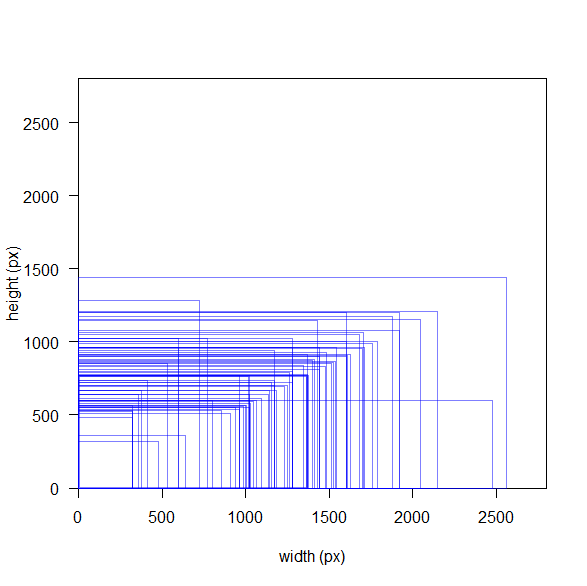
\includegraphics[height=\textheight]{images/devicesizes.png}
\end{center}
}


\frame{

\frametitle{Non-textual Manipulations}

\small

\begin{itemize}\itemsep0.5em
\item Images can work well
\item Standalone or embedded in a text or question
\item<2-> Examples
	\begin{itemize}\footnotesize
	\item<2-> Kalmoe \& Gross\footnote{``Cueing Patriotism, Prejudice, and Partisanship in the Age of Obama: Experimental Tests of U.S. Flag Imagery Effects in Presidential Elections.'' \textit{Political Psychology}: in press.} measure impact of patriotic cues on candidate support by showing images of candidates with and without flags
	\item<3-> Subliminal primes possible, depending on software
	\item<4-> Lots of recent examples of facial manipulation
	\end{itemize}

\end{itemize}

}

\frame{

\frametitle{Example\footnote{Iyengar et al. 2010. ``Do Explicit Racial Cues Influence Candidate Preference? The Case of Skin Complexion in the 2008 Campaign.'' Working paper.}}

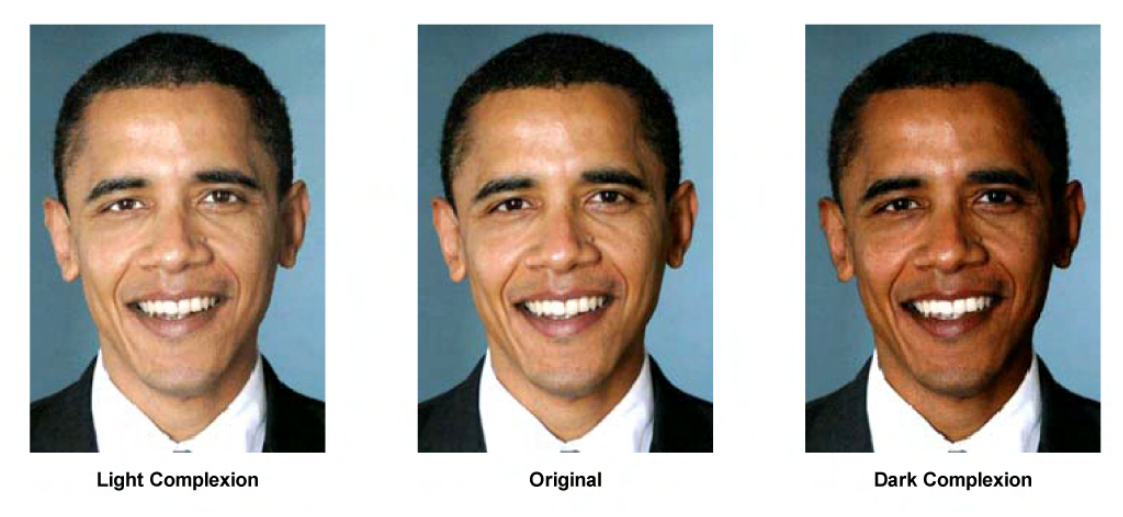
\includegraphics[width=\textwidth]{images/IyengarMessingBailenson}

}

\frame{

\frametitle{{\normalsize Example\footnote{Laustsen \& Petersen. 2016. ``Winning Faces vary by Ideology.'' \textit{Political Communication} 33(2): 188--211.}}}

\begin{center}
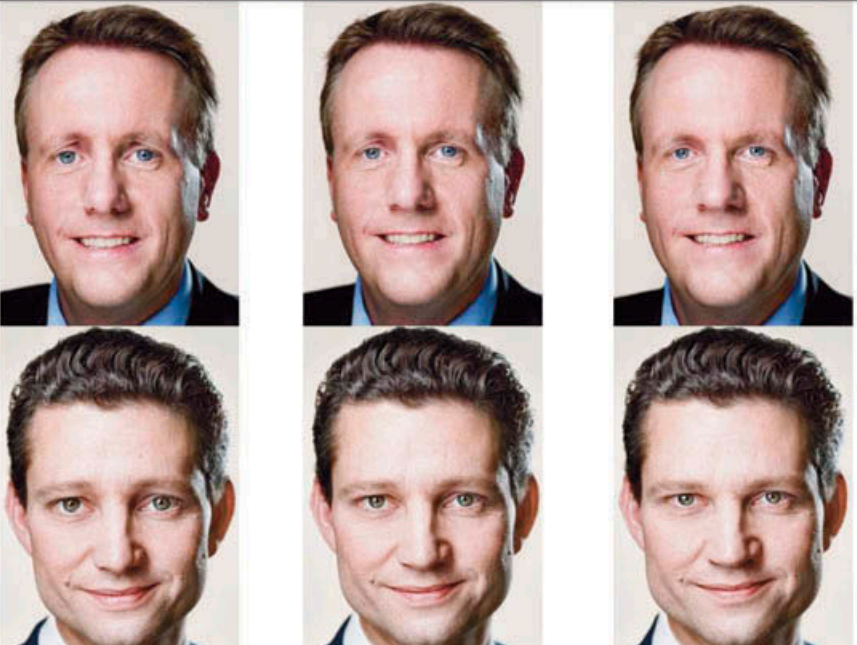
\includegraphics[width=\textwidth, trim={0cm 0cm 0cm 9cm}, clip]{images/laustsen}
\end{center}
}

\frame{
\frametitle{{\normalsize Example\footnote{Bailenson et al. 2006. ``Transformed Facial Similarity as a Political Cue: A Preliminary Investigation.'' \textit{Political Psychology} 27(3): 373--385.}}}

\begin{center}
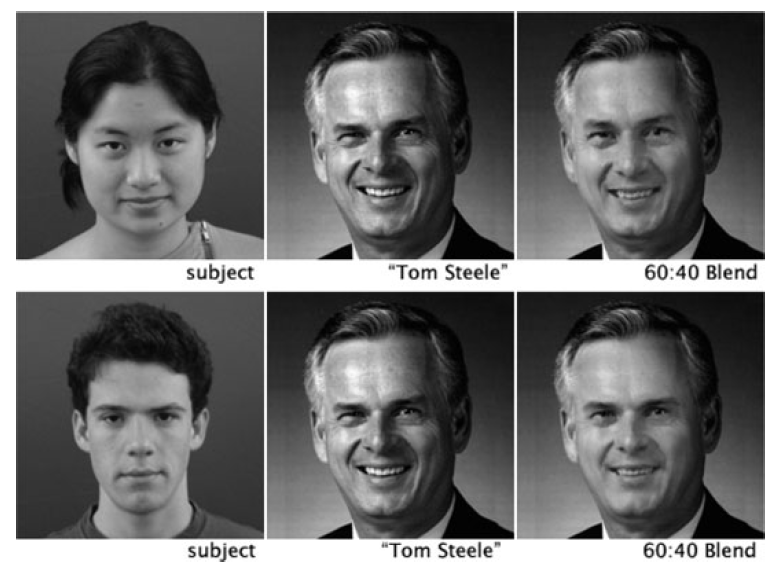
\includegraphics[width=\textwidth, trim={0cm 7.7cm 0cm 0cm}, clip]{images/BailensonGarlandIyengar}
\end{center}
}




\frame{

\frametitle{{\normalsize Audio \& Video manipulations}}

\small

\begin{itemize}\itemsep-0.2em
\item Problematic for same reasons as long texts
\item<2-> Best practices
	\begin{itemize}\footnotesize
	\item Keep it short
	\item Have the video play automatically
	\item Disallow survey progression
	\item Control and validate
	\end{itemize}
\item<3->Examples
	\begin{itemize}
	\item Television Advertisements\footnote{Vavreck. 2007 ``The Exaggerated Effects of Advertising on Turnout: The Dangers of Self-Reports.'' \textit{Quarterly Journal of Political Science} 2: 325--343.} 
	\item News Programs\footnote{Mutz. 2007. ``Effects of `In-Your-Face' Television Discourse on Perceptions of a Legitimate Opposition.'' \textit{American Political Science Review} 101(4): 621--635.}
	\end{itemize}	
\end{itemize}

}




\frame{
\frametitle{``Task'' Designs}

\begin{itemize}\itemsep0.5em
\item Task designs ask respondents to perform a task
\item Often developed for laboratory settings
\item<2-> Most common example: writing something
\item<3-> Can be problematic:
	\begin{itemize}
	\item Time-intensive
	\item Invites drop-off
	\item Compliance problems
	\end{itemize}
\end{itemize}

}


\againframe{ambivalentpartisan}



\questions


\subsection[More Designs]{More Advanced Designs}
\frame{\tableofcontents[currentsection,currentsubsection,subsubsectionstyle=hide]}

\frame{

\frametitle{Beyond Simple Designs}

\begin{enumerate}\itemsep1em
\item Factorial designs
\item Sensitive question designs
\item Conjoint designs
\item Multi-component designs
	\begin{itemize}
	\item Over-time measurement/randomization
	\item Field--survey combinations
	\end{itemize}
\end{enumerate}
}



\frame{

\frametitle{Sensitive Item Designs}

\begin{itemize}\itemsep1em
\item Randomization can be used to measure something

\item List experiments
	\begin{itemize}
	\item Randomly present lists of items of varying length
	\item Difference in count of items supported is prevalence of sensitive attitude/behavior
	\end{itemize}

\item Randomized response
	\begin{itemize}
	\item Present a sensitive question
	\item Use a randomization device to dictate whether the respondent answers the sensitive question or something else
	\end{itemize}
\end{itemize}
}

\frame{

\frametitle{{\normalsize List Experiments \footnote{Kuklinski et al. 1997. ``Racial Prejudice and Attitudes Toward Affirmative Action.'' \textit{American Journal of Political Science} 41(2): 402--419.}}}

\small

Now I'm going to read you three things that sometimes make people angry or upset. After I read all three, just tell me \textit{how many} of them upset you. I don't want to know which ones. just \textit{how many}.

\footnotesize

\begin{enumerate}
\item the federal government increasing the tax on gasoline
\item professional athletes getting million-dollar salaries
\item large corporations polluting the environment
\item<2-> \textbf{a black family moving in next door}
\end{enumerate}

}


\frame{

\frametitle{Randomized Response\footnote{Blair, Imai, and Zhou. 2015. ``Design and Analysis of the Randomized Response Technique.'' \textit{JASA} 110(511): 1304--19.}}

\begin{itemize}\itemsep1em
\item Example:

{\footnotesize
Here is a bag; in it there are stones from the game `Go,' some colored black and others white. Please take one stone out, and see by yourself what color it is, black or white. Don't let me know whether it is black or white, but be sure you know which it is.\\

If you take a black one, answer the question: ``Have you ever had an induced abortion?''\\

If you take a white one, answer the question: ``Were you born in the lunar year of the horse?'
}

\item Considerations:
	\begin{itemize}
	\item Can use any randomization device
	\item Can be cognitively complex
	\end{itemize}
\end{itemize}




}



\frame{}





% CONJOINTS
\frame{

\frametitle{Conjoint Analysis}

\begin{itemize}\itemsep1em
\item Surveys measure \textit{stated} preferences
\item Conjoint analysis involves measuring \textit{revealed} preferences based upon a series of forced-choice decisions

	\begin{itemize}
	\item Present respondents with pairs of ``profiles'' containing many \textit{features}
	\item Force respondents to choose which of the two they prefer
	\end{itemize}

\item Estimate \textit{relative} importance of features of each profile

\item Randomization of profile features gives differences in preferences across attributes a causal meaning 

\end{itemize}

}


\frame{

\frametitle{Advantages/Disadvantages}

\begin{itemize}\itemsep1em
\item Advantages

\begin{itemize}
\item Reduces ``cheap talk'' results
\item Lower social desirability biases
\item Mimics real-world decisions
\item Revealed preferences are causally interpretable
\end{itemize}

\item Disadvantages

\begin{itemize}
\item More cognitively complex for respondents than traditional polling
\item No straightforward ``\% support'' statistics
\end{itemize}

\end{itemize}

}

\frame{

\frametitle{Structure of Conjoints}

\begin{itemize}\itemsep1em
\item Three examples:
	\begin{enumerate}
	\item Policy preference on Brexit negotiations
	\item Choice of BBC Director General
	\item Choice of a lodger
	\end{enumerate}

\item All are binary, forced-choice designs 

\item Analysis is all focused on AMCEs or subgroup AMCEs

	\begin{itemize}
	\item Estimated using OLS dummy variable regression
	\end{itemize}
\end{itemize}

}


\frame{

\frametitle{{\normalsize Conjoint 1: Brexit Negotiations}}

\begin{center}
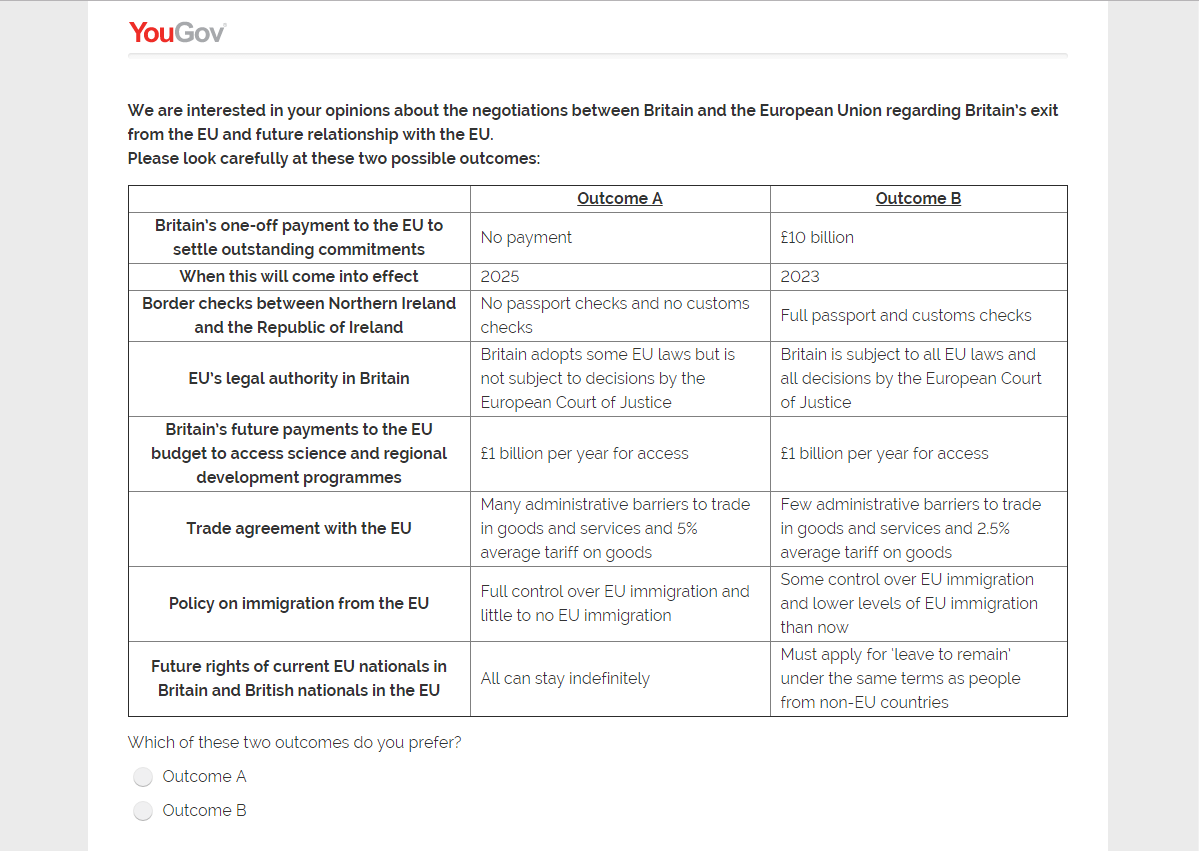
\includegraphics[height=.9\textheight]{images/brexit-conjoint-screenshot}
\end{center}
}


\frame{

\frametitle{{\normalsize Conjoint 2: BBC Director}}

\small
Imagine that you are deciding who to appoint as the next Director General of the BBC. You have received the following information about two applicants and need to make a decision between them.\\

\vspace{1em}

\begin{columns}\footnotesize
\begin{column}{.5\textwidth}
 - Tom\\
 - 68 years old\\
 - Has worked 21 years for the BBC\\
 - Has a degree from the University of Oxford\\
 - Didn't vote at the 2017 election\\
 - Voted Remain in the EU referendum\\
 - Former lawyer
\end{column}
\begin{column}{.5\textwidth}
 - Claire\\
 - 35 years old\\
 - Has never worked for the BBC\\
 - Has a PhD from the University of Exeter\\
 - Voted Conservative at the 2017 election\\
 - Didn't vote in the EU referendum\\
 - Former television producer
\end{column}
\end{columns}

\vspace{1em}

Which of the two applicants would you prefer as the next Director General of the BBC?

}


\frame{

\frametitle{{\normalsize Conjoint 3: Lodger}}

\small
Imagine that you have a spare room that you want to rent out to a lodger. You have received the following information about two possible lodgers and need to make a decision between them.\\

\vspace{1em}

\begin{columns}\footnotesize
\begin{column}{.5\textwidth}
 - James\\
 - 19 years old\\
 - Full-time student\\
 - Helps out at the local Anglican church\\
 - Didn't vote at the 2017 election\\
 - Voted Remain in the EU referendum\\
 - Likes watching rugby
\end{column}
\begin{column}{.5\textwidth}
 - Becky\\
 - 35 years old\\
 - Works for a private company\\
 - Volunteers at an Oxfam shop\\
 - Voted Conservative at the 2017 election\\
 - Didn't vote in the EU referendum\\
 - Likes playing videogames
\end{column}
\end{columns}

\vspace{1em}

Which of the two lodgers would you prefer? 

}



\frame{
\frametitle{AMCEs}

Statistic of interest is the \textit{average marginal component effect} (AMCE), which is the causal effect of each level of each feature on support for an overall profile.

\vspace{1em}

We can estimate this using (dummy variable) OLS, assuming:

\begin{itemize}
\item Full randomization of attributes and randomized pairing of profiles
\item Even presentation of levels w/in features
\item No profile ordering effects
\end{itemize}

}

\frame{
\begin{center}
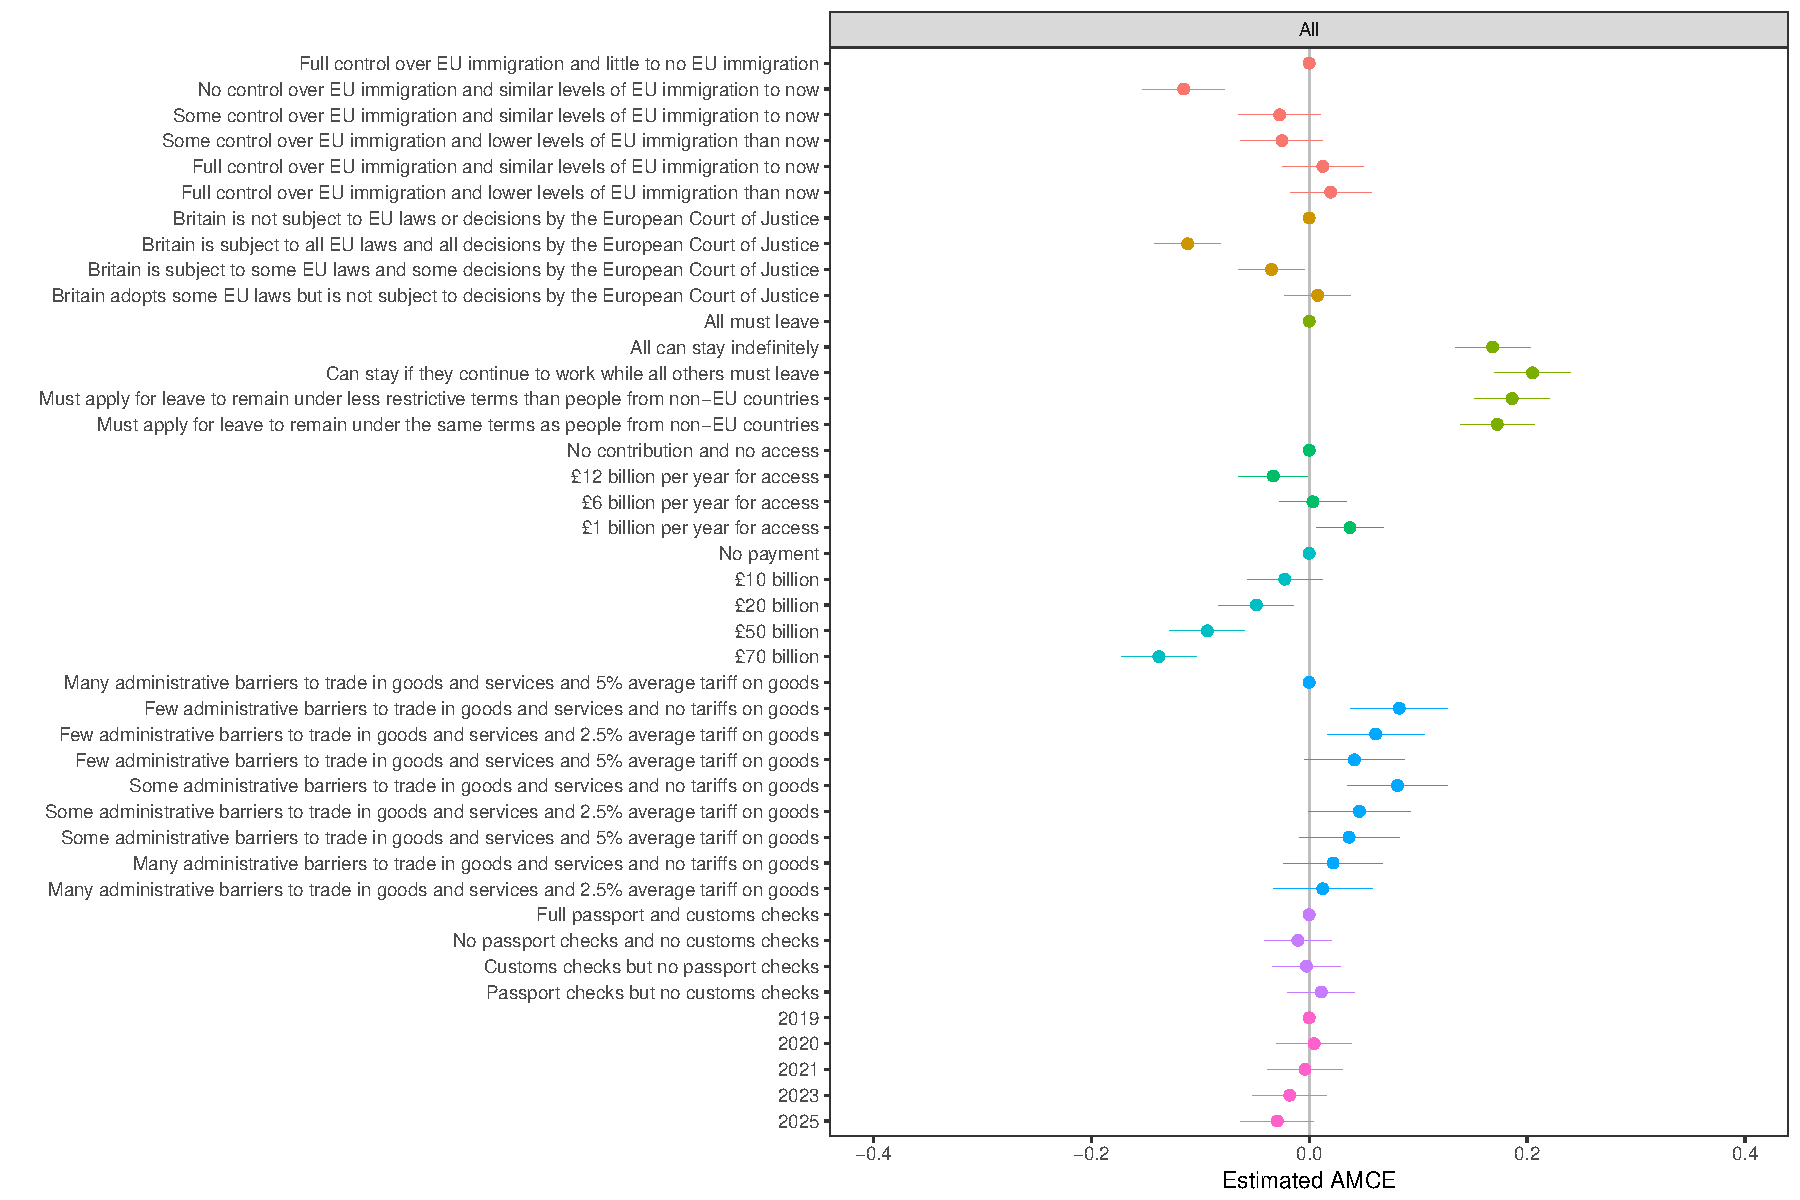
\includegraphics[width=\textwidth]{images/brexit-conjoint}
\end{center}
}

\frame{
\begin{center}
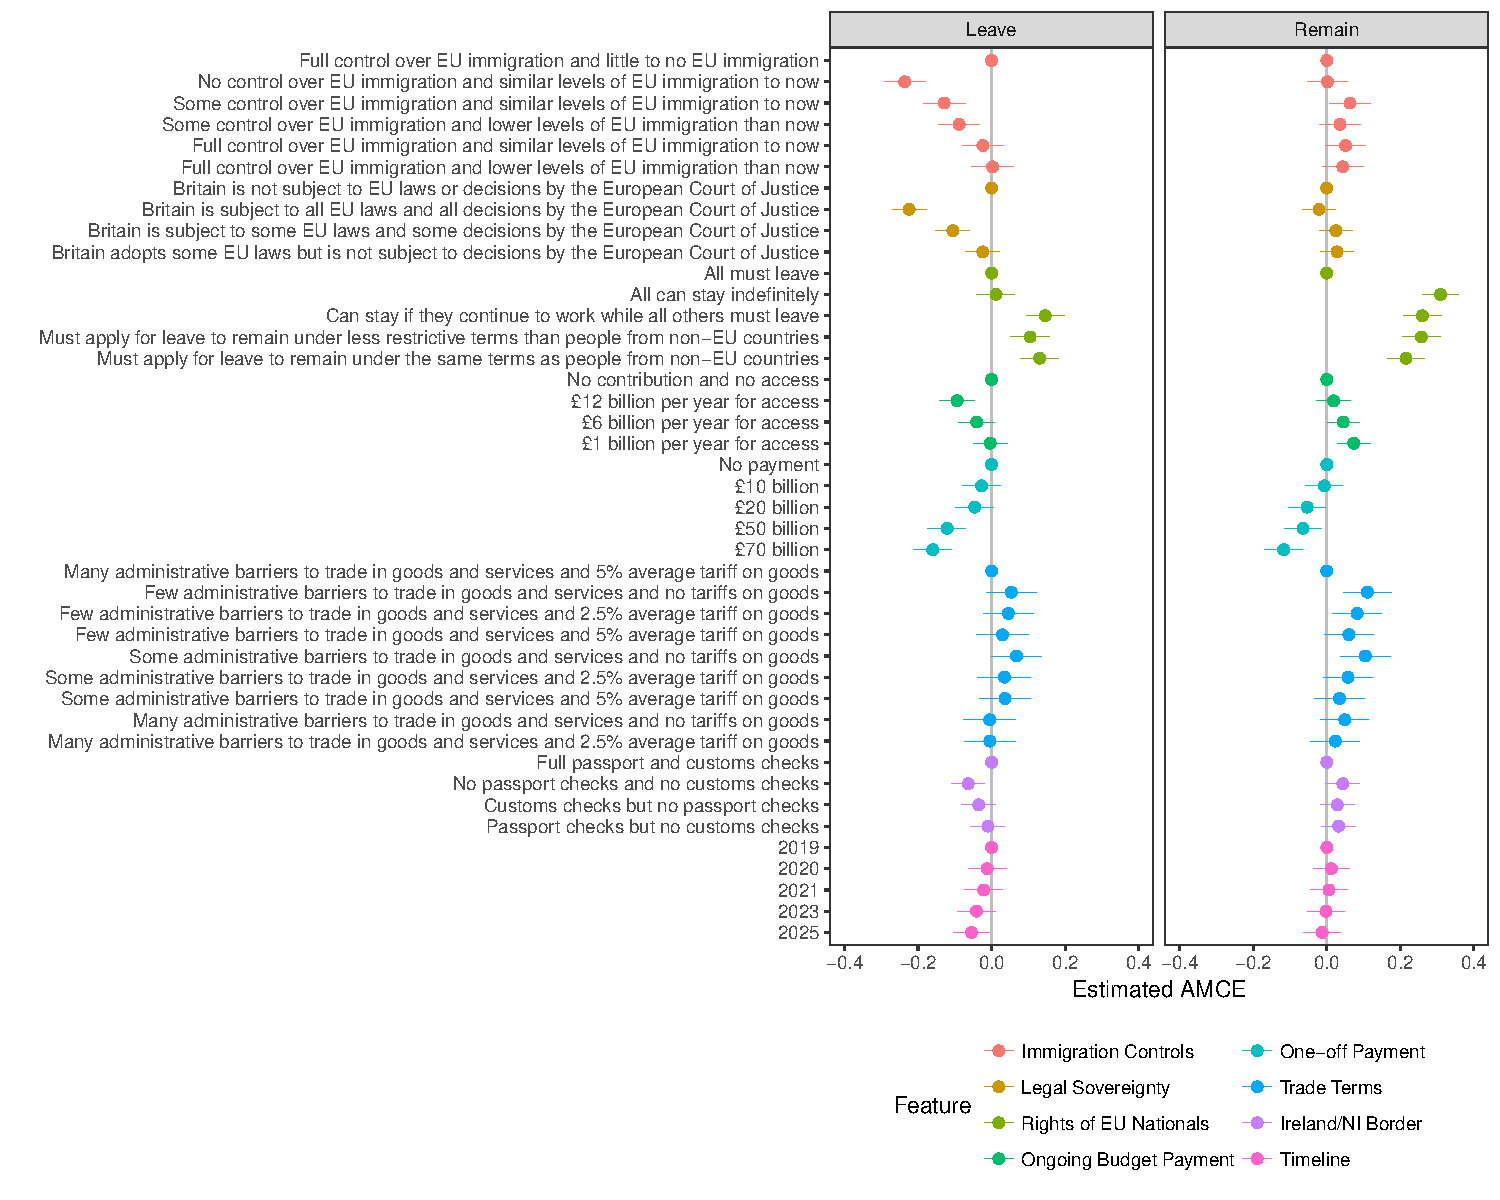
\includegraphics[height=\textheight]{images/brexit-conjoint-split}
\end{center}
}

\frame{
\begin{center}
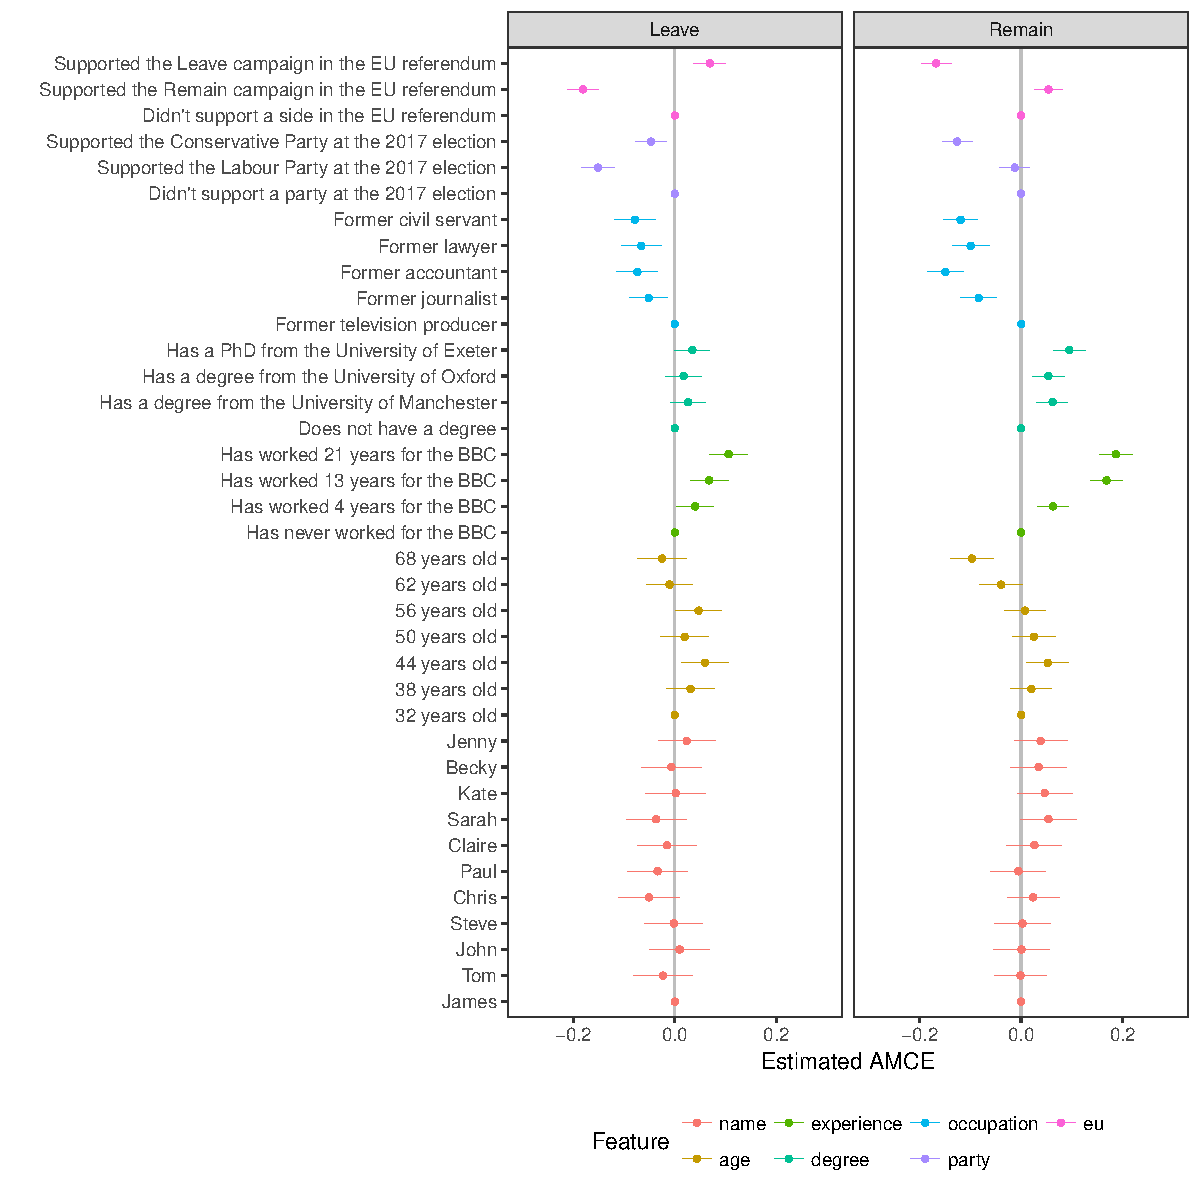
\includegraphics[height=\textheight]{images/conjoint-bbc-1}
\end{center}
}

\frame{
\begin{center}
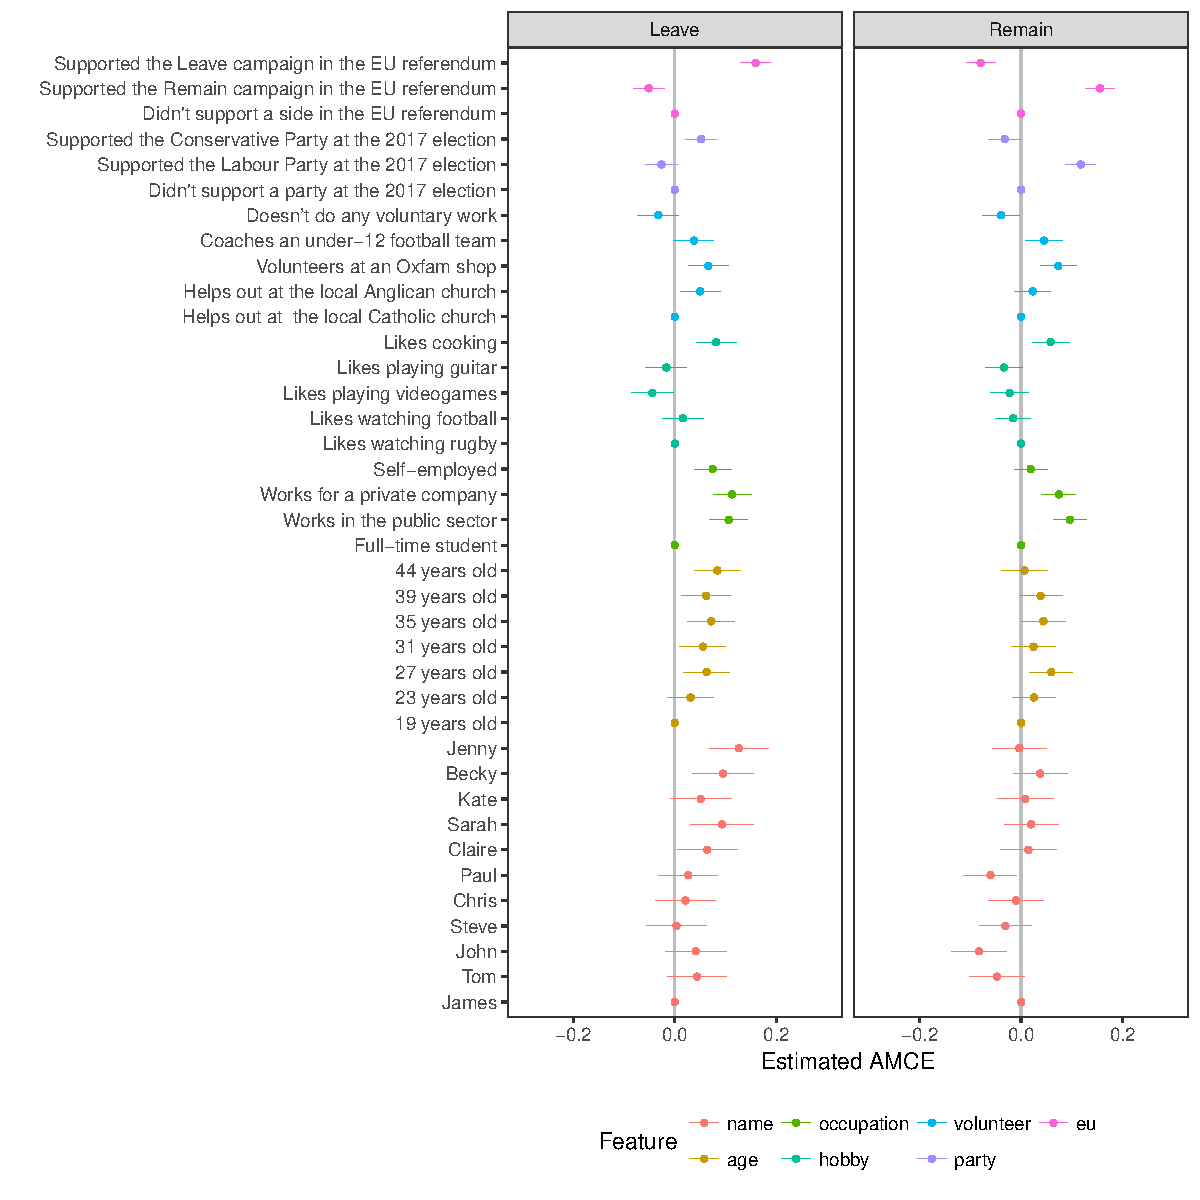
\includegraphics[width=\textheight]{images/conjoint-lodger-1}
\end{center}
}


\frame{

\frametitle{Implementing a Conjoint}

\begin{itemize}\itemsep1em
\item Hope someone else can do it for you!

	\begin{itemize}
	\item Requires programming
	\item Not possible to manually create all possible combinations
	\end{itemize}

\item Strezhnev et al.'s tool:\\
{\small \url{https://scholar.harvard.edu/astrezhnev/conjoint-survey-design-tool}}

\item Qualtrics using Javascript:\\
{\small \url{https://github.com/leeper/conjoint-example}}
\end{itemize}

}


\frame{}


\questions




\section[Challenges]{Challenges and Criticisms}
\frame{\tableofcontents[currentsection,subsubsectionstyle=hide]}


\subsection{Participant Recruitment}
\frame{\tableofcontents[currentsection,currentsubsection,subsubsectionstyle=hide]}

\frame{

\frametitle{How do we find participants?}

\begin{itemize}\itemsep1em
\item Volunteers
	\begin{itemize}
	\item Volunteer Science
	\item In-house subject pool
	\end{itemize}

\item Paid crowdworkers
	\begin{itemize}
	\item Prolific Academic
	\item Mechanical Turk
	\item Crowdflower
	\end{itemize}

\item ``Representative'' samples
	\begin{itemize}
	\item Big players: YouGov, TNS, Gallup, Nielsen, GfK
	\item Others: Kantar, SSI, Lucid
	\end{itemize}
\end{itemize}

}

\frame{
\frametitle{SUTO Framework}
\begin{itemize}\itemsep0.5em
\item Cronbach (1986) talks about generalizability in terms of UTO
\item Shadish, Cook, and Campbell (2001) speak similarly of:
	\begin{itemize}
	\item \textbf{S}ettings
	\item \textbf{U}nits
	\item \textbf{T}reatments
	\item \textbf{O}utcomes
	\end{itemize}
\item External validity depends on all of these
\end{itemize}
}


\frame{
\begin{columns}[t]
\begin{column}{0.5\textwidth}
	\begin{block}{Population}
		\begin{itemize}
		\item Setting
		\item Units
		\item Treatments
		\item Outcomes
		\end{itemize}
	\end{block}
\end{column}
\begin{column}{0.5\textwidth}
	\begin{block}{Your Study}
		\begin{itemize}
		\item Setting
		\item Units
		\item Treatments
		\item Outcomes
		\end{itemize}
	\end{block}
\end{column}
\end{columns}

\vspace{0.5em}

\small

\only<2->{In your study, how do these correspond?\\}
\only<3->{\hspace{5.7em} how do these differ?\\}
\only<4->{\hspace{5.7em} do these differences matter?\\}

}

\frame{
\frametitle{Common Differences}
\begin{itemize}\itemsep1em
\item Most common thing to focus on is demographic representativeness
	\begin{itemize}
	\item Sears (1986): ``students aren't real people''
	\item \href{http://www.slate.com/articles/health_and_science/science/2013/05/weird_psychology_social_science_researchers_rely_too_much_on_western_college.html}{Western, educated, industrialized, rich, democratic (WEIRD) psychology participants}
	\end{itemize}
\item<2-> But do those characteristics actually matter?
\item<3-> Shadish, Cook, and Campbell tell us to think about:
	\begin{itemize}
	\item Surface similarities
	\item Ruling out irrelevancies
	\item Making discriminations
	\item Interpolation/extrapolation
	\end{itemize}
\end{itemize}
}

\frame{
\begin{center}
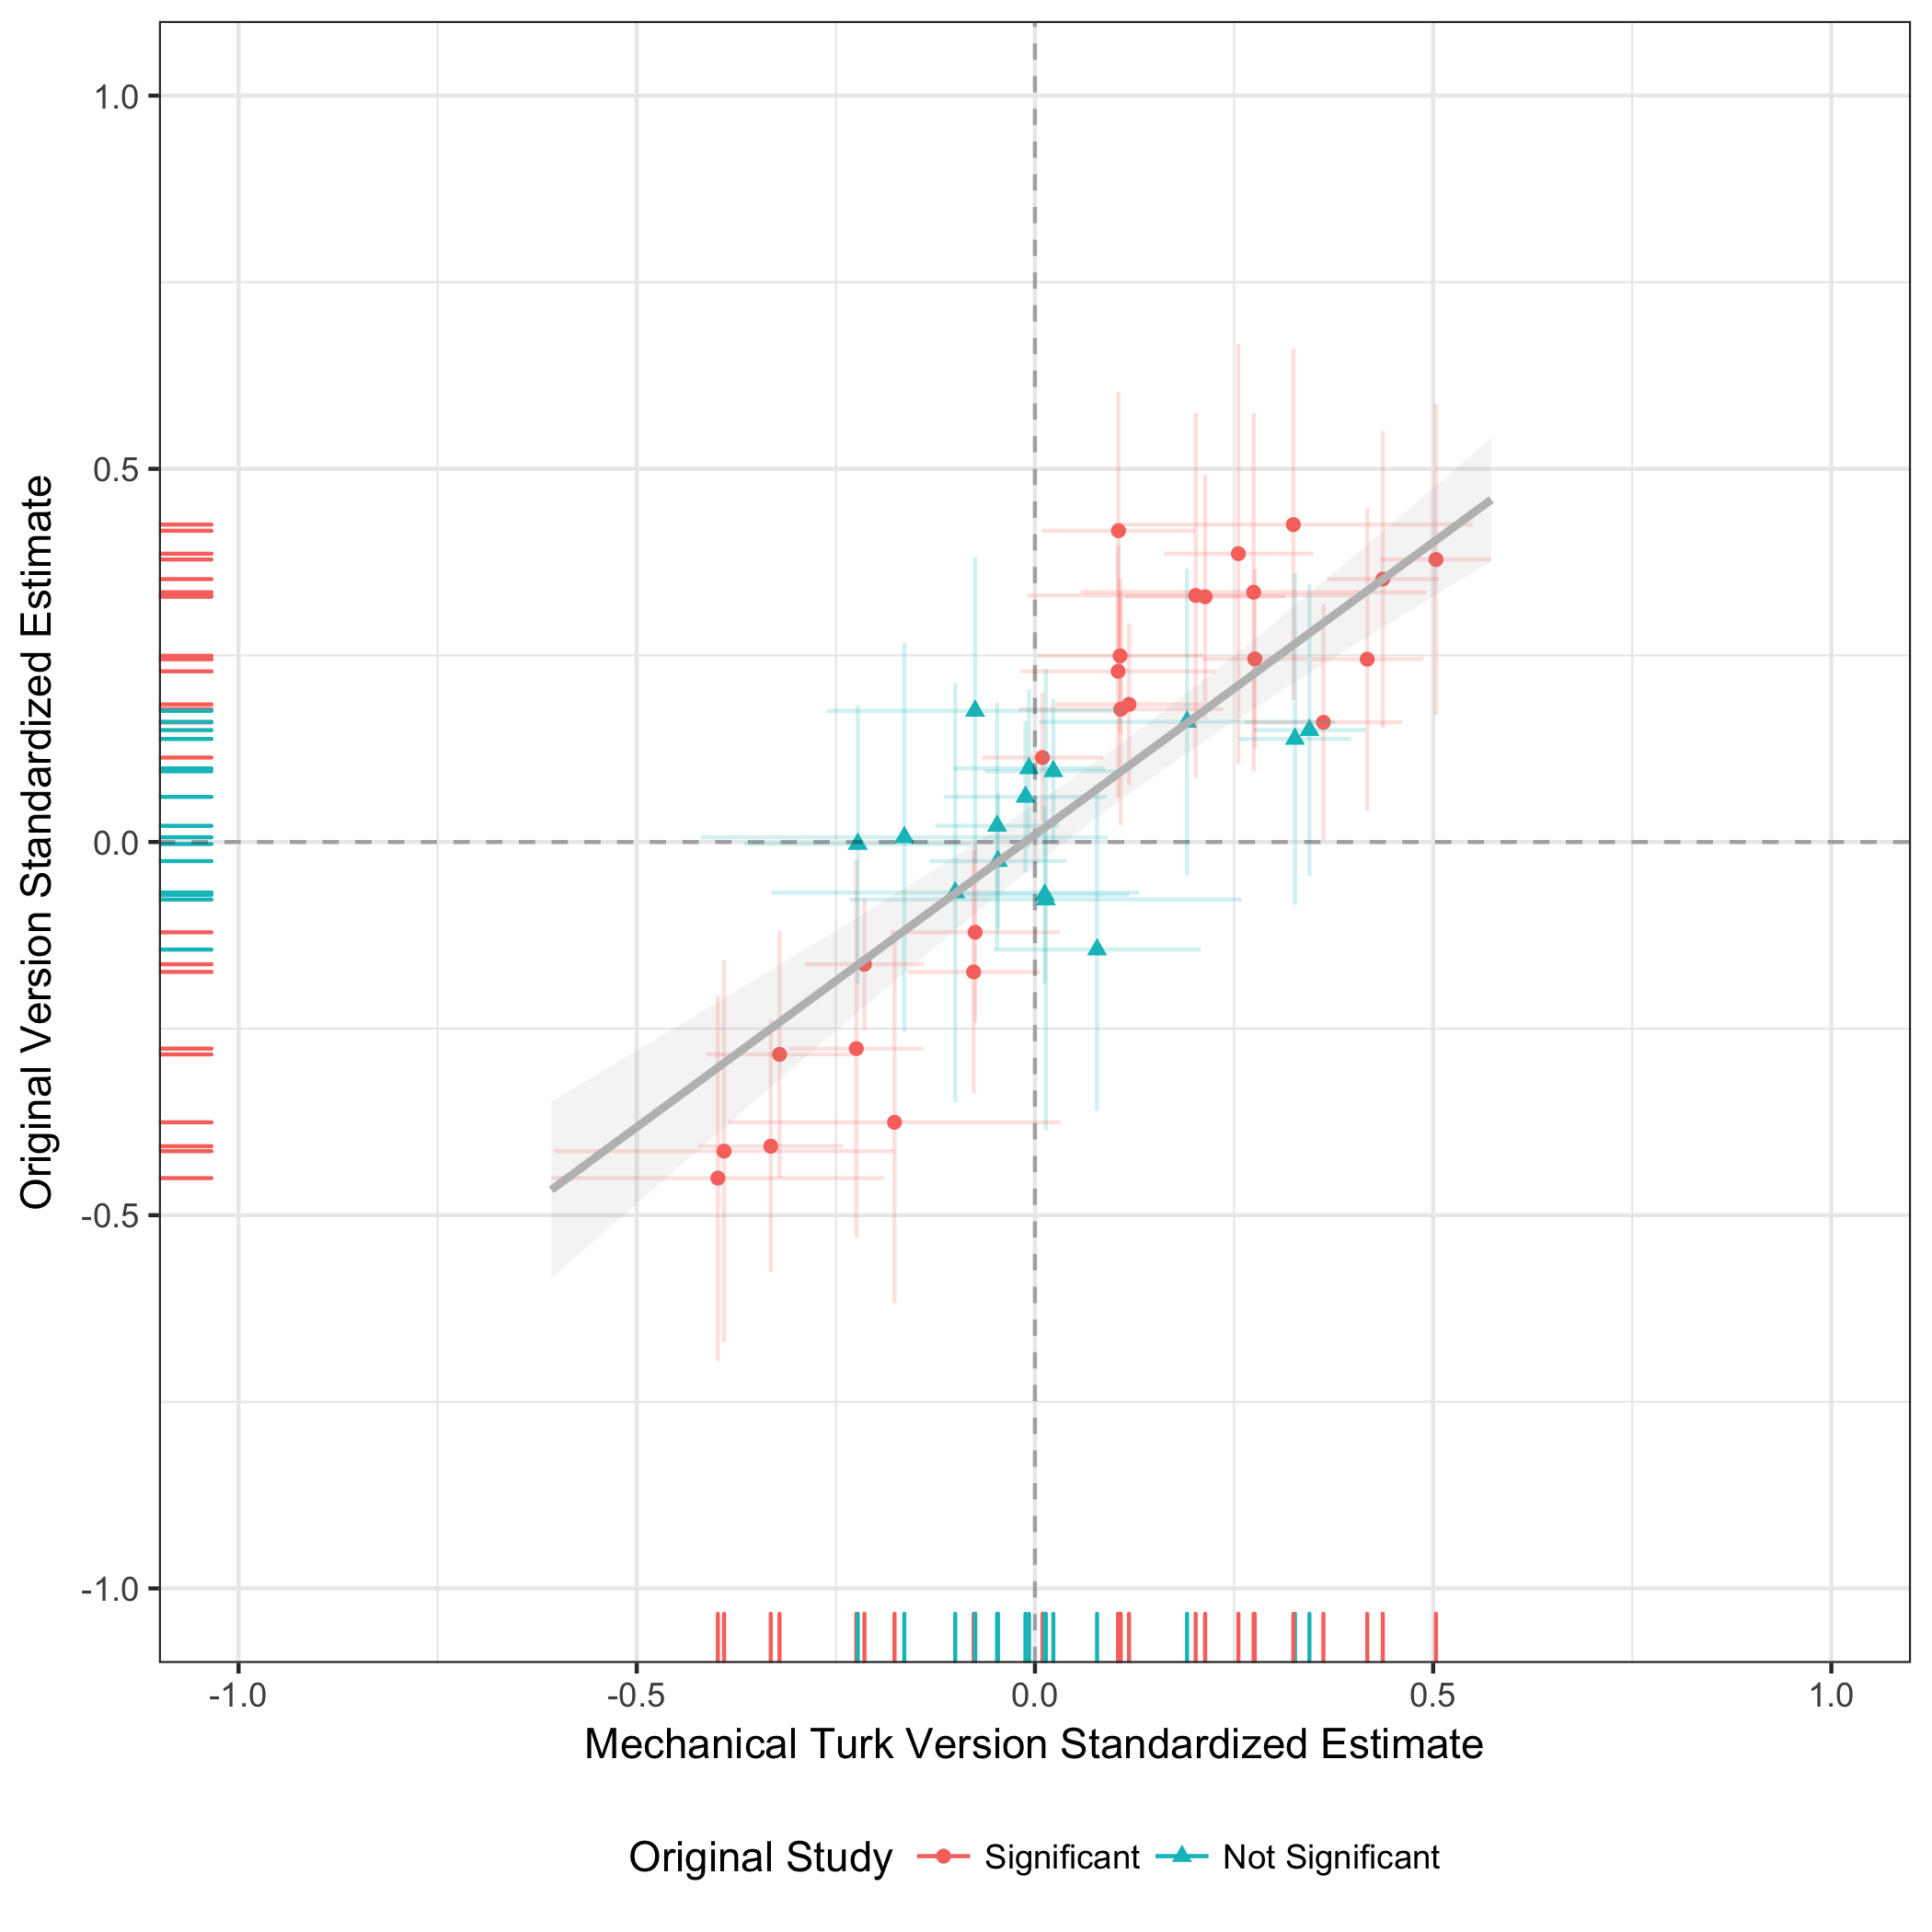
\includegraphics[height=\textheight]{images/coppock_et_al-1}
\end{center}
}

\frame{
\begin{center}
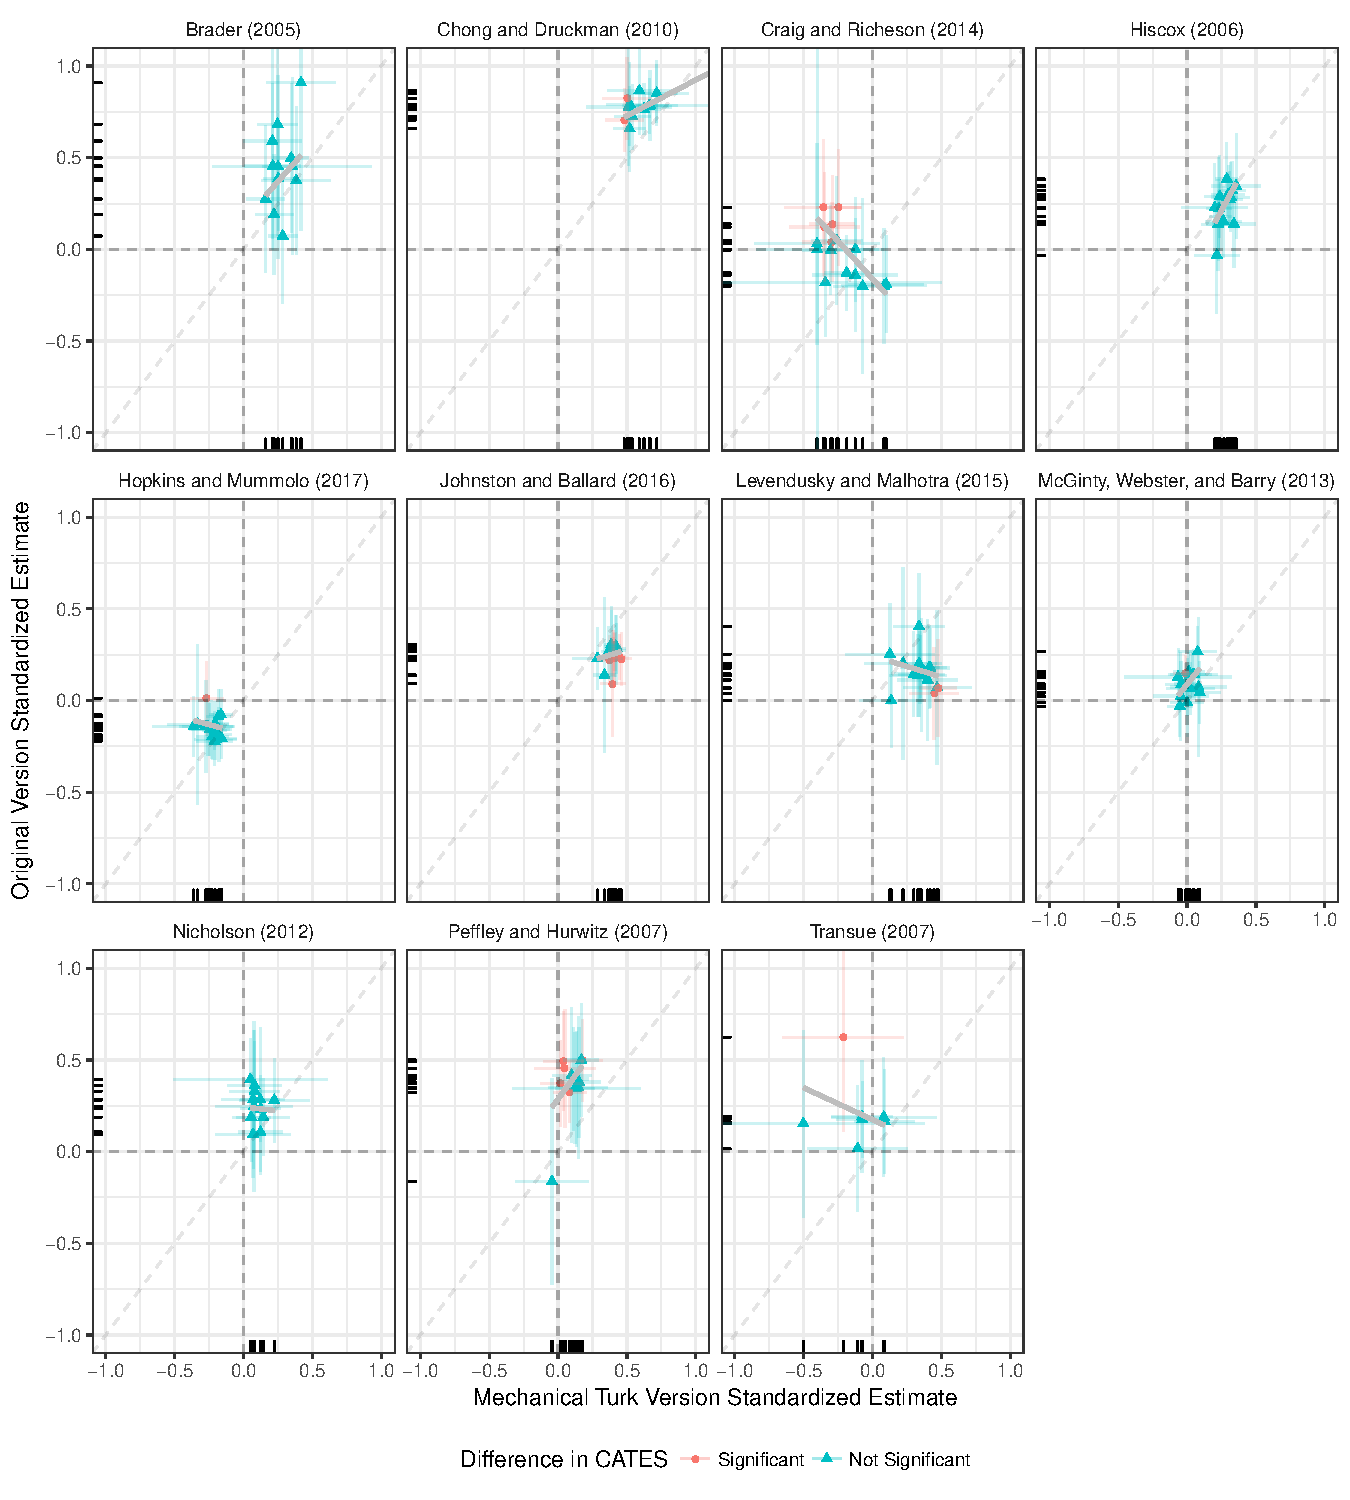
\includegraphics[height=\textheight]{images/coppock_et_al-2}
\end{center}
}

\questions

\subsection{Attention and Satisficing}
\frame{\tableofcontents[currentsection,currentsubsection,subsubsectionstyle=hide]}

\frame{

One final issue with unit-related sources of heterogeneity is how we handle or analyze survey-experimental data where we think participants misbehaved.

\vspace{1em}

\only<2->{This falls into a couple of broad categories:

\begin{itemize}
\item Noncompliance
\item Inattention
\item Survey Satisficing
\end{itemize}
}
}

\frame{

How should we deal with respondents that appear to not be paying attention, not ``taking'' the treatment, or not responding to outcome measures?

\begin{enumerate}
\item Keep them
\item Throw them away
\end{enumerate}

}

\frame{

\frametitle{Best Practice: Pre-Analysis Protocol}

\begin{itemize}\itemsep0.5em
\item Excluding respondents based on survey behavior is one of the easiest ways to ``p-hack'' an experimental dataset
	\begin{itemize}
	\item Inattention, satisficing, etc. will tend to reduce the size of the SATE
	\end{itemize}
\item So regardless of how you handle these respondents, these should be decisions that are made \textit{pre-analysis}
\end{itemize}

}


\frame[label=exclusion]{

\frametitle{{\normalsize When are you excluding participants?}}

    \begin{columns}[T]
    \begin{column}[T]{5cm}
        \begin{block}{\rule[-0.6ex]{0pt}{2.5ex}Pre-Treatment}
            \begin{itemize}\itemsep0.2em
                \item<2-> \hyperlink{satisficing}{Satisficing behaviors}
                \item<3-> Inattention
                \item<4-> Covariate-based selection
                \item<5-> Pretreated
            \end{itemize}
        \end{block}
    \end{column}
    \begin{column}[T]{5cm}
        \begin{block}{\rule[-0.6ex]{0pt}{2.5ex}Post-Treatment}
            \begin{itemize}\itemsep0.5em
                \item<6-> Speeding on treatment
                \item<7-> ``Failing'' a manipulation check
                \item<8-> Drop-off
            \end{itemize}
        \end{block}
    \end{column}
    \end{columns}

}


\frame{

\frametitle{Pre-Treatment Exclusion}

\begin{itemize}\itemsep0.5em
\item This is totally fine from a causal inference perspective
\item<2-> Advantages:
	\begin{itemize}
	\item Focused on engaged respondents
	\item Likely increase impact of treatment
	\end{itemize}
\item<3-> Disadvantages:
	\begin{itemize}
	\item Changing definition of sample (and thus population)
	\end{itemize}
\end{itemize}

}


\frame{

\frametitle{Post-Treatment Exclusion}

This is much more problematic because it involves controlling for a \textit{post-treatment} variable

}

\frame<1-3>[label=posttreatment]{

\begin{center}
\begin{tikzpicture}[>=latex',circ/.style={draw, shape=circle, node distance=5cm, line width=1.5pt}]
    \draw (0,0) node[left, text width=3cm, align=center] (X) {Information};
    \draw (5,0) node[right, text width=2cm, align=center] (Y) {Opinion};
    \draw<1-3>[->] (X) -- (Y);
    \draw[->] (4,-4) node[below, text width=3cm, align=center] (E) {Etc.} -- (Y);
	\draw<2-> (1,-2) node[text width=3cm, align=center] (M) {Manipulation Check};
	\draw<2-4>[->,thick,red] (X) -- (M);
    \draw<2-4>[->,thick,red] (M) -- (Y);
    \draw<3>[->] (E) -- (M);
\end{tikzpicture}
\end{center}

\small 
\only<2>{Risk that estimate of $\beta_1$ is diminished because effect is being carried through the manipulation check.}
\only<3>{Introduction of ``collider bias'' wherein values of the manipulation check are affected by other factors.}
}





\frame[label=posttreatment2]{

\frametitle{Post-Treatment Exclusion}

\small

\begin{itemize}\itemsep0.5em
\item Any post-treatment exclusion is problematic and should be avoided
\item<2-> Can estimate a LATE
	\begin{itemize}\footnotesize
	\item Interpretation: Effect of manipulation check among those whose value of the check can be changed by the treatment manipulation
	\end{itemize}
\item<3-> Non-response or attrition is the same as researcher-imposed exclusion
	\begin{itemize}\footnotesize
	\item Not problematic if MCAR
	\item Nothing really to be done if caused by treatment
	\end{itemize}
\end{itemize}

}

\againframe<3-4>{posttreatment}

\againframe<2->{posttreatment2}


\questions

\frame[label=satisficing]{
\frametitle{Apparent Satisficing}
\begin{itemize}\itemsep0.5em
\item Some common measures:
	\begin{itemize}
	\item ``Straightlining''
	\item Non-differentiation
	\item Acquiescence
	\item Nonresponse
	\item DK responding
	\item Speeding
	\end{itemize}
\item Difficult to detect and distinguish from ``real'' responses
\end{itemize}
}

\frame{
\frametitle{Metadata/Paradata}
\begin{itemize}\itemsep1em
\item<1-> Timing
	\begin{itemize}
	\item Some survey tools will allow you to time page
	\item Make a prior rules about dropping participants for speeding
	\end{itemize}
\item<2-> Mousetracking or eyetracking
	\begin{itemize}
	\item Mousetracking is unobtrusive
	\item Eyetracking requires participants opt-in
	\end{itemize}
\item<3-> Record focus/blur browser events
\end{itemize}
}

\frame{
\frametitle{Direct Measures}
\begin{itemize}\itemsep1em
\item How closely have you been paying attention to what the questions on this survey actually mean?
\item<2-> While taking this survey, did you engage in any of the following behaviors? Please check all that apply.
	\begin{itemize}
	\item Use your mobile phone
	\item Browse the internet
	\item \dots
	\end{itemize}
\end{itemize}
}



\frame{
\frametitle{{\normalsize Instructional Manipulation Check}}

\small

\only<2>{Do you agree or disagree with the decision to send British forces to fight ISIL in Syria? }We would like to know if you are reading the questions on this survey. If you are reading carefully, please ignore this question, do not select any answer below, and click ``next'' to proceed with the survey.\\

\vspace{0.5em}

\footnotesize
Strongly disagree\\
Somewhat disagree\\
Neither agree nor disagree\\
Somewhat agree\\
Strongly agree\\

\vspace{1em}
\only<2>{\hyperlink{exclusion}{\beamerbutton{Return}}}
}



\frame{

\frametitle{{\normalsize Treatment Noncompliance}}

\begin{itemize}\itemsep0.5em
\item Definition:\\{\small ``when subjects who were assigned to receive the treatment go untreated or when subjects assigned to the control group are treated'' \footnote{Gerber \& Green. 2012. \textit{Field Experiments}, p.132.}}
\item<2-> Several strategies
	\begin{itemize}
	\item ``As treated'' analysis
	\item ``Intention to treat'' analysis
	\item Estimate a LATE
	\end{itemize}
\end{itemize}

}

\frame{
\frametitle{{\normalsize Analyzing Noncompliance}}

\small

\begin{itemize}\itemsep0.5em
\item If noncompliance only occurs in one group, it is \textit{asymmetric} or \textit{one-sided}
\item We can ignore non-compliance and analyze the ``intention to treat'' effect, which will underestimate our effects because some people were not treated as assigned: $ITT = \overline{Y}_1 - \overline{Y}_0$
\item<2-> We can use ``instrumental variables'' to estimate the ``local average treatment effect'' (LATE) for those that complied with treatment: $LATE = \frac{ITT}{\% Compliant}$
\end{itemize}
}

\frame{
	\frametitle{{\large Local Average Treatment Effect}}
	\small
	\begin{itemize}\itemsep0.2em
	\item IV estimate is \textit{local} to the variation in $X$ that is due to variation in $D$
	\item This matters if effects are \textit{heterogeneous}
	\item LATE is effect for those who \textit{comply}
	\item Four subpopulations:
		\begin{itemize}\footnotesize
		\item Compliers: $X = 1$ only if $D = 1$
		\item Always-takers: $X = 1$ regardless of $D$
		\item Never-takers: $X = 0$ regardless of $D$
		\item Defiers: $X = 1$ only if $D = 0$
		\end{itemize}
	\item Exclusion restriction! Monotonicity!
	\end{itemize}
}

\questions




\subsection{Use of Covariates}
\frame{\tableofcontents[currentsection,currentsubsection,subsubsectionstyle=hide]}

\frame{

\frametitle{Block Randomization I}

{\small \textbf{Stratification:Sampling::Blocking:Experiments}}

\small

\begin{itemize}\itemsep0.5em
\item<2-> Basic idea: randomization occurs within strata defined before treatment assignment
\item<3-> CATE is estimate for each stratum; aggregated to SATE
\item<4-> Why?
	\begin{itemize}
	\item Eliminate chance imbalances
	\item Optimized for estimating CATEs
	\item More precise SATE estimate
	\end{itemize}
\end{itemize}

}

\begin{frame}[fragile]

\begin{center}
\begin{tabular}{lcccccccc}
Exp. & \multicolumn{4}{c}{Control} & \multicolumn{4}{c}{Treatment} \\ \midrule
1 & M & M & M & M & F & F & F & F \\
2 & M & M & M & F & M & F & F & F \\
3 & M & M & F & F & M & M & F & F \\
4 & M & F & F & F & M & M & M & F \\
5 & F & F & F & F & M & M & M & M \\ \bottomrule
\end{tabular}
\end{center}


{\scriptsize
\begin{verbatim}
# population of men and women
pop <- rep(c("Male", "Female"), each = 4)

# randomly assign into treatment and control
split(sample(pop, 8, FALSE), c(rep(0,4), rep(1,4)))
\end{verbatim}
}

\end{frame}

\frame{

\begin{center}

\begin{tabular}{rrrr}
Obs. & $X_{1i}$ & $X_{2i}$ & $D_i$ \\ \midrule
1 & Male & Old & 0 \\
2 & Male & Old & 1 \\  \midrule
3 & Male & Young & 1 \\
4 & Male & Young & 0 \\ \midrule
5 & Female & Old & 1 \\
6 & Female & Old & 0 \\ \midrule
7 & Female & Young & 0 \\
8 & Female & Young & 1 \\ \bottomrule
\end{tabular}
\end{center}

}

\frame[label=blocking2]{

\frametitle{Block Randomization II}

\begin{itemize}
\item Blocking ensures ignorability of all covariates used to construct the blocks
\item Incorporates covariates explicitly into the \textit{design}
\item<2-> When is blocking \textit{statistically} useful?
	\begin{itemize}
	\item<3-> If those covariates affect values of potential outcomes, blocking reduces the variance of the SATE
	\item<4-> Most valuable in small samples
	\item<5-> Not valuable if all blocks have similar potential outcomes
	\end{itemize}
\end{itemize}

}



\frame{

\frametitle{Statistical Properties I}

\small

Complete randomization:\\
$$SATE = \frac{1}{n_1}\sum Y_{1i} - \frac{1}{n_0}\sum Y_{0i}$$

\vspace{2em}

Block randomization:\\
$$SATE_{blocked} = \sum_{1}^{J} \left( \dfrac{n_j}{n} \right)  (\widehat{CATE}_j)$$

}


\frame{

\begin{center}

\begin{tabular}{rrrrrr}
Obs. & $X_{1i}$ & $X_{2i}$ & $D_i$ & $Y_i$ & CATE \\ \midrule
1 & Male & Old & 0 & 5 & \multirow{2}{*}{\onslide<2->{5}} \\
2 & Male & Old & 1 & 10 \\  \midrule
3 & Male & Young & 1 & 4 & \multirow{2}{*}{\onslide<3->{3}} \\
4 & Male & Young & 0 & 1 \\ \midrule
5 & Female & Old & 1 & 6 & \multirow{2}{*}{\onslide<4->{4}} \\
6 & Female & Old & 0 & 2 \\ \midrule
7 & Female & Young & 0 & 6 & \multirow{2}{*}{\onslide<5->{3}} \\
8 & Female & Young & 1 & 9 \\ \bottomrule
\end{tabular}
\end{center}

}

\frame{

\frametitle{SATE Estimation}

\begin{align*}
SATE &= \left(\dfrac{2}{8}*5\right) + \left(\dfrac{2}{8}*3\right) + \left(\dfrac{2}{8}*4\right) + \left(\dfrac{2}{8}*3\right) \\ \vspace{1em}
&= 3.75
\end{align*}

\onslide<2->{The blocked and unblocked estimates are the same here because $Pr(Treatment)$ is constant across blocks and blocks are all the same size.}

}

\frame{

\frametitle{SATE Estimation}

\small

\begin{itemize}
\item We can use weighted regression to estimate this in an OLS framework
\item Weights are the inverse prob. of being treated w/in block
\begin{itemize}
\item Pr(Treated) by block: $p_{ij} = Pr(D_i = 1 | J=j) $
\item Weight (Treated): $ w_{ij} = \dfrac{1}{p_{ij}} $
\item Weight (Control): $ w_{ij} = \dfrac{1}{1-p_{ij}} $
\end{itemize}
\end{itemize}

}


\frame{

\frametitle{Statistical Properties II}

\small

Complete randomization:\\
$$\widehat{SE}_{SATE} = \sqrt{\dfrac{\widehat{Var}(Y_0)}{n_0} + \dfrac{\widehat{Var}(Y_1)}{n_1}}$$

\vspace{1em}

Block randomization:\\
$$\widehat{SE}_{SATE_{blocked}} = \sqrt{\sum_{1}^{J} \left( \dfrac{n_j}{n} \right)^2  \widehat{Var}{(SATE_j)}}$$

\only<2->{When is the blocked design more efficient?}

}


\frame{

\frametitle{Practicalities}

\begin{itemize}\itemsep0.5em
\item Blocked randomization only works in exactly the same situations where stratified sampling works
	\begin{itemize}
	\item Need to observe covariates pre-treatment in order to block on them
	\item Work best in a panel context
	\end{itemize}
\item In a single cross-sectional design that might be challenging
	\begin{itemize}
	\item Some software can block ``on the fly''
	\end{itemize}
\end{itemize}


}


\questions





\section{Conclusion}
\frame{\tableofcontents[currentsection,subsubsectionstyle=hide]}

\frame{}

\frame{

\Large

\begin{center}
Quiz time!
\end{center}

}


\frame{
\frametitle{Compliance}

\large

\begin{enumerate}\itemsep0.5em
\item<1-> What is compliance?
\item<2-> How can we analyze experimental data when there is noncompliance?
\end{enumerate}
}

\frame{
\frametitle{Balance testing}

\normalsize

\begin{enumerate}\itemsep0.5em
\item<1-> What does randomization ensure about the composition of treatment groups?
\item<2-> What can we do if we find a covariate imbalance between groups?
\item<3-> How can we avoid this problem entirely?
\end{enumerate}
}


\frame{
\frametitle{Nonresponse and Attrition}

\large

\begin{enumerate}\itemsep0.5em
\item<1-> Do we care about outcome nonresponse in experiments?
\item<2-> How can we analyze experimental data when there is outcome nonresponse or post-treatment attrition?
\end{enumerate}
}


\frame{
\frametitle{Manipulation checks}

\large

\begin{enumerate}\itemsep0.5em
\item<1-> What is a manipulation check? What can we do with it?
\item<2-> What do we do if some respondents ``fail'' a manipulation check?
\end{enumerate}
}



\frame{
\frametitle{Null effects}

\large

\begin{enumerate}\itemsep0.5em
\item<1-> What should we do if we find our estimated $\widehat{SATE} = 0$?
\item<2-> What does it mean for an experiment to be \textit{underpowered}?
\item<3-> What can we do to reduce the probability of obtaining an (unwanted) ``null effect''?
\end{enumerate}
}


\frame{
\frametitle{Representativeness}

\large

\begin{enumerate}\itemsep0.5em
\item<1-> Under what conditions is a design-based, probability sample necessary for experimental inference?
\item<2-> What kind of causal inferences can we draw from an experiment on a descriptively unrepresentative sample?
\end{enumerate}
}

\frame{
\frametitle{Types of Experiments}

\large

\begin{enumerate}\itemsep0.5em
\item<1-> What are the three basic ways to construct experimental manipulations?
\item<2-> What are some useful and common paradigms for survey experiments?
\end{enumerate}
}

\frame{
\frametitle{Conjoints}

\large

\begin{enumerate}\itemsep0.5em
\item<1-> What are conjoints useful for?
\item<2-> How do we correctly analyze a conjoint experimental design?
\end{enumerate}
}


\frame{
\frametitle{Peer Review}

\large

\begin{enumerate}\itemsep0.5em
\item<1-> What should we do if a peer reviewer asks us to ``control'' for covariates in the analysis?
\item<2-> What should we do if a peer reviewer asks us to include or exclude particular respondents from the analysis?
\end{enumerate}
}


\questions

\frame{

\frametitle{Learning Outcomes}

\small

By the end of the day, you should be able to\dots

\begin{enumerate}
\item<2-> Explain how to analyze experiments quantitatively.
\item<3-> Explain how to design experiments that speak to relevant research questions and theories.
\item<4-> Evaluate the uses and limitations of several common survey experimental paradigms.
\item<5-> Identify practical issues that arise in the implementation of experiments and evaluate how to anticipate and respond to them.
\end{enumerate}

}


\frame{
	\frametitle{Wrap-up}
	\begin{itemize}
	\item Thanks to all of you!
	\item Stay in touch (\href{mailto:t.leeper@lse.ac.uk}{t.leeper@lse.ac.uk})
	\item Good luck with your research!
	\end{itemize}
}


\frame{}

\appendix

\frame{\tableofcontents}

\section{Protocols}

\frame{

\frametitle{{\normalsize TESS has ``Open Protocols''}}

Protocol is the complete planning document for how to design, implement, and analyze an experiment.\footnote{Thomas J. Leeper. 2011. ``The Use of Protocol in the Design and Reporting of Experiments.'' \textit{The Experimental Political Scientist}.}

\small

\begin{enumerate}\itemsep-0.2em
\item Theory/hypotheses
\item Instrumentation
	\begin{itemize}
	\item Manipulation(s)
	\item Outcome(s)
	\item Covariate(s)
	\item Manipulation check(s)
	\end{itemize}
\item Sampling
\item Implementation
\item Analysis
\end{enumerate}
}

\frame{

\frametitle{Why bother writing a protocol?}

\begin{itemize}\itemsep0.5em
\item<2-> Be clear to yourself what you're trying to do before you do it
\item<3-> Assess the literature for best practices
\item<4-> Highlight areas in need of pilot testing
\item<5-> Economize questionnaire development
\item<6-> Study preregistration
\end{itemize}

}


\section{Effect Heterogeneity}

\frame{
\frametitle{{\large Detecting Effect Heterogeneity}}

Always block if you expect heterogeneity!

\begin{itemize}\itemsep0.5em
\item QQ-plots: Suggestive evidence
\item Regression using treatment-by-covariate interactions
\item<2-> (Replication and meta-analysis)
\end{itemize}

}



\frame{

\frametitle{Suggestive Evidence}

We can never know $Var(TE_i)$! \onslide<2->{But\dots}

\begin{itemize}\itemsep0.5em
\item<2-> Quantile-quantile plots
	\begin{itemize}
	\item<3-> Compare the distribution of $Y_0$'s to distribution of $Y_1$'s
	\item<3-> If homogeneity, a vertical shift in $Y_1$'s
	\item<3-> If heterogeneity, a slope $\neq$ 1
	\end{itemize}
\item<4-> Equality of variance tests
	\begin{itemize}
	\item<4-> If homogeneity, variance should be equal
	\item<4-> If heterogeneity, variances should differ
	\end{itemize}
\end{itemize}

}

\begin{frame}[fragile]

\frametitle{QQ Plots}

{\scriptsize
\begin{verbatim}
# y_0 data
set.seed(1)
n <- 200
y0 <- rnorm(n) + rnorm(n, 0.2)

# y_1 data (homogeneous effects)
y1a <- y0 + 2 + rnorm(n, 0.2)
# y_1 data (heterogeneous effects)
y1b <- y0 + rep(0:1, each = n/2) + rnorm(n, 0.2)

qqplot(y0, y1a, pch=19, xlim=c(-3,5), ylim=c(-3,5), asp=1)
curve((x), add = TRUE)
qqplot(y0, y1b, pch=19, xlim=c(-3,5), ylim=c(-3,5), asp=1)
curve((x), add = TRUE)
\end{verbatim}

}

\end{frame}


\frame{

\begin{center}
\only<1>{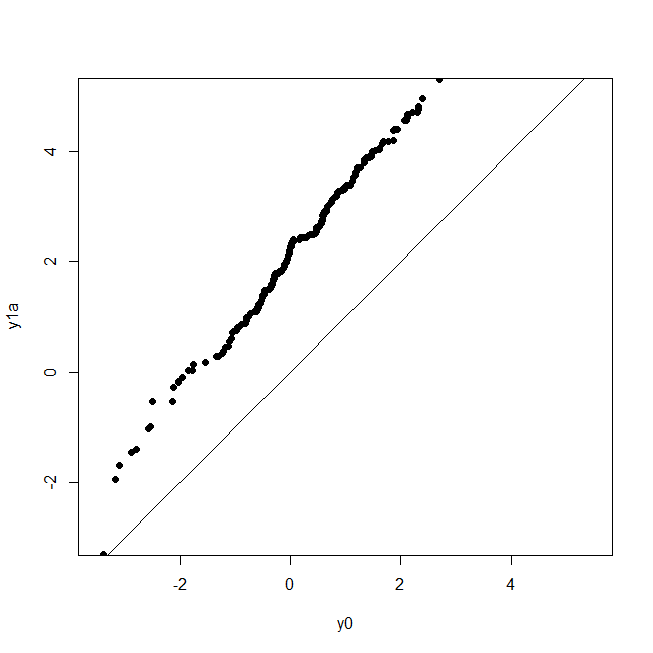
\includegraphics[height=\textheight]{images/qqplot1}}
\only<2>{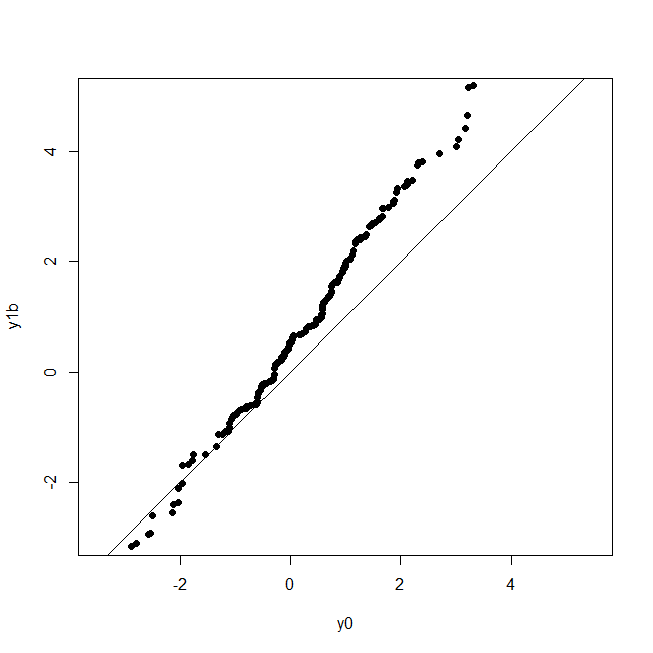
\includegraphics[height=\textheight]{images/qqplot2}}
\end{center}

}

\begin{frame}[fragile]

\frametitle{Equality of Variance tests}

\footnotesize

\begin{verbatim}
> var.test(y0, y1a)

        F test to compare two variances

data:  y0 and y1a
F = 0.60121, num df = 199, denom df = 199, 
  p-value = 0.0003635
alternative hypothesis: 
  true ratio of variances is not equal to 1
95 percent confidence interval:
 0.4549900 0.7944289
sample estimates:
ratio of variances 
         0.6012131 
\end{verbatim}

\end{frame}

\begin{frame}[fragile]

\frametitle{Equality of Variance tests}

\footnotesize

\begin{verbatim}
> var.test(y0, y1b)

        F test to compare two variances

data:  y0 and y1b
F = 0.53483, num df = 199, denom df = 199,
  p-value = 1.224e-05
alternative hypothesis:
  true ratio of variances is not equal to 1
95 percent confidence interval:
 0.4047531 0.7067133
sample estimates:
ratio of variances 
         0.5348312
\end{verbatim}

\end{frame}


\questions


\frame{\frametitle{Regression Estimation}}

\frame{

\frametitle{{\normalsize Aside: Regression Adjustment in Experiments, Generally}}

\begin{itemize}\itemsep0.5em
\item Recall the general advice that we do not need covariates in the regression to ``control'' for omitted variables (because there are none)
\item Including covariates can reduce variance of our SATE by explaining more of the variation in $Y$
\end{itemize}

}

\frame{

\frametitle{Scenario}

Imagine two regression models. Which is correct?

\begin{enumerate}
\item Mean-difference estimate of SATE is ``not significant''
\item Regression estimate of SATE, controlling for sex, age, and education, is ``significant''
\end{enumerate}

\onslide<2->{This is a small-sample dynamic, so make these decisions pre-analysis!}

}

\frame{

\frametitle{{\normalsize Treatment-Covariate Interactions}}

\normalsize

\begin{itemize}
\item The regression paradigm allows us to estimate CATEs using interaction terms
	\begin{itemize}
	\item $X$ is an indicator for treatment
	\item $M$ is an indicator for possible moderator
	\end{itemize}
\item<2-> SATE: $Y = \beta_0 + \beta_1 X + e$
\item<3-> CATEs: $$Y = \beta_0 + \beta_1 X + \beta_2 M + \beta_3 X*M + e$$
	\begin{itemize}
	\item<4-> Homogeneity: $\beta_3 = 0$
	\item<4-> Heterogeneity: $\beta_3 \neq 0$
	\end{itemize}

\end{itemize}

}


\section{Advanced Designs}

\section[More Designs]{Beyond One-Shot Designs}
\frame{\tableofcontents[currentsubsection,subsubsectionstyle=hide]}

\frame{

\frametitle{{\normalsize Beyond One-shot Designs}}


\begin{itemize}\itemsep0.5em
\item Surveys can be used as a measurement instrument for a field treatment or a manipulation applied in a different survey panel wave
	\begin{enumerate}
	\item Measure effect duration in two-wave panel
	\item Solicit pre-treatment outcome measures in a two-wave panel
	\item Measure effects of field treatment in post-test only design
	\item Randomly encourage field treatment in pre-test and measure effects in post-test
	\end{enumerate}
\item<2-> Problems? Compliance \& nonresponse
\end{itemize}

}

\frame{

\frametitle{{\normalsize I. Effect Duration}}

\begin{itemize}\itemsep0.5em
\item Use a two- (or more-) wave panel to measure duration of effects
	\begin{itemize}
	\item T1: Treatment and outcome measurement
	\item T2+: Outcome measurement
	\end{itemize}
\item Two main concerns
	\begin{itemize}
	\item Attrition
	\item Panel conditioning
	\end{itemize}
\end{itemize}

}

\frame{

\frametitle{{\normalsize II. Within-Subjects Designs}}

\small

\begin{itemize}
\item Estimate treatment effects as a difference-in-differences
\item Instead of using the post-treatment mean-difference in $Y$ to estimate the causal effect, use the difference in pre-post differences for the two groups:
	\begin{align*}
	(\hat{Y}_{0,t+1} - \hat{Y}_{0,t}) - (\hat{Y}_{j,t+1} - \hat{Y}_{j,t})
	\end{align*}
\item<2-> Advantageous because variance for paired samples decreases as correlation between $t_0$ and $t_1$ observations increases
\end{itemize}

}


\frame{
	\begin{center}
	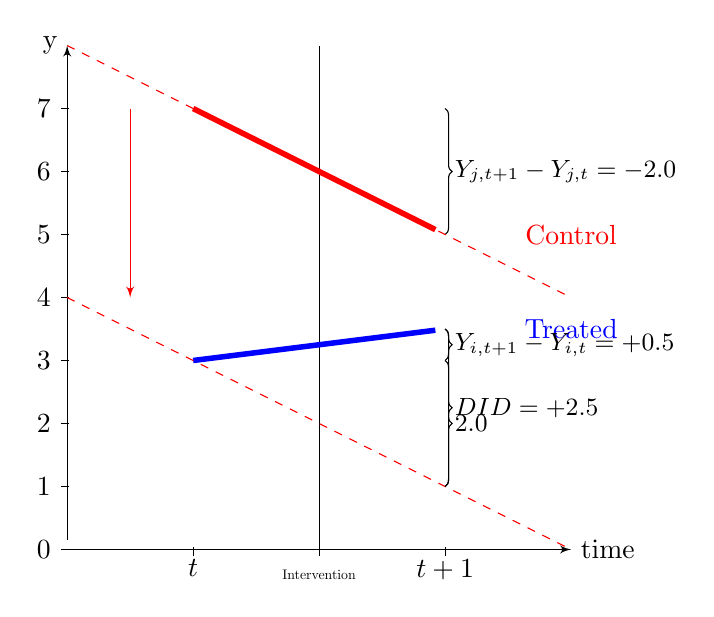
\begin{tikzpicture}[>=latex', scale=0.8]
        \draw[->] (0,0) node (origin) {}  -- (8,0) node[right] (xaxis) {time};
        \draw[->] (origin) -- (0,8) node[left] (yaxis) {y};
        % x ticks
        \foreach \x in {2,4,6}
        	\draw (\x,1pt) -- (\x,-3pt) node[anchor=north] {};
        \draw (2,0) node[below] (before) {$t$};
        \draw (6,0) node[below] (after) {$t+1$};
        \draw (4,-0.25) node[below, scale=0.5] (IV) {Intervention};
        % y ticks
        \foreach \y in {0,...,7}
             \draw (1pt,\y) -- (-3pt,\y) node[anchor=east] {$\y$};
        % intervention
        \draw (4,0) -- (4,8);

        % line
        \draw<2-> (6,3.5) node (tr) {};
        \draw<3-> (6,5) node (ctrl) {};
        \draw<2-3>[blue] (8,3.5) node (trlab) {Treated};
        \draw<3-3>[red] (8,5) node (ctrllab) {Control};        
        \draw<2->[blue, line width=2pt] (2,3) -- (tr);
        \draw<3->[red, line width=2pt] (2,7) -- (ctrl);
        
        % diffs
        \draw<4-6>[right,decorate,decoration={brace,mirror}] 
        	(6,3) -- (6,3.5) node[right, pos=0.5] (idiff) {\small $Y_{i,t+1} - Y_{i,t} = +0.5$};
        \draw<4-6>[right,decorate,decoration={brace}] 
            (6,7) -- (6,5) node[right, pos=0.5] (jdiff) {\small $Y_{j,t+1} - Y_{j,t} = -2.0$};
        
        % trends
        \draw<5-6>[red,->] (1,7) -- (1,4);
        \draw<5->[red, dashed] (0,8) -- (8,4);
        \draw<5->[red, dashed] (0,4) -- (8,0);
        \draw<6>[right,decorate,decoration={brace}] 
            (6,3) -- (6,1) node[right, pos=0.5] (idiff2) {\small $2.0$};
        \draw<7>[right,decorate,decoration={brace}] 
            (6,3.5) -- (6,1) node[right, pos=0.5] (idiff2) {\small $DID = +2.5$};
                        
        
    \end{tikzpicture}
    \end{center}
}


\frame{

	\frametitle{{\normalsize Threats to Validity}}
	
	\small
	
	As soon as time comes into play, we have to worry about threats to validity.\footnote{Shadish, Cook, and Campbell (2002)}
	
	\begin{enumerate}
	\item<2-> History (simultaneous cause)
	\item<3-> Maturation (time trends)
	\item<4-> Testing (observation changes respondents)
	\item<5-> Instrumentation (changing operationalization)
	\item<6-> Instability (measurement error)
	\item<7-> Attrition
	\end{enumerate}
}






\frame{

\frametitle{{\normalsize III. Randomized Field Treatment}}

\small

\begin{itemize}\itemsep-0.2em
\item Examples:
	\begin{enumerate}
	\item<2-> Citizens randomly sent a letter by post encouraging them to reduce water usage
	\item<3-> Different local media markets randomly assigned to receive different advertising
	\end{enumerate}
\item<4-> Survey is used to measure outcomes, when treatment assignment is already known
\item<5-> Issues
	\begin{itemize}
	\item<6-> Nonresponse
	\item<6-> Noncompliance
	\end{itemize}
\end{itemize}

}

\frame{

\frametitle{{\normalsize IV. Treatment Encouragement}}

\small

\begin{itemize}\itemsep-0.2em
\item Design:
	\begin{itemize}
	\item T1: Encourage treatment
	\item T2: Measure effects
	\end{itemize}
\item Examples:
	\begin{enumerate}
	\item Albertson and Lawrence\footnote{Albertson \& Lawrence. 2009. ``After the Credits Roll.'' \textit{American Politics Research} 37(2): 275--300. \href{http://doi.org/10.1177/1532673X08328600}{10.1177/1532673X08328600}.}
	\end{enumerate}
\item<2-> Issues
	\begin{itemize}
	\item<3-> Nonresponse
	\item<3-> Noncompliance
	\end{itemize}
\end{itemize}

}


\end{document}
